% !TeX root = ../../Skript.tex
\cohead{\Large\textbf{Produktform}}
\fakesubsection{Produktform}
Hat eine ganzrationale Funktion \(f(x)\) vom Grad \(n\) genauso viele Nullstellen wie ihr Grad, so kann man sie in der Produktform darstellen:

\(f(x)=a\left(x-x_1 \right)^{n_1} \left(x-x_2 \right)^{n_2}\left(x-x_3 \right)^{n_3} \cdots, \quad a\neq 0, \quad n_1,\ n_2,\ n_3,\ldots\in\N\)

Wie auch bei der Produktform der quadratischen Funktionen lassen sich die Nullstellen einfach ablesen. Auch der Leitkoeffizient und der Grad lassen sich leicht bestimmen:
\begin{itemize}\large
	\item[\textcolor{loes}{\textbullet}] \textcolor{loes}{\(x_1,\ x_2,\ x_3,\ldots\): Nullstellen der Funktion}
	\item[\textcolor{loes}{\textbullet}]  \textcolor{loes}{\(n_1,\ n_2,\ n_3,\ldots\): Zu den Nullstellen gehörige Vielfachheiten (VFH) der Nullstellen}
	\item[\textcolor{loes}{\textbullet}]  \textcolor{loes}{\(a\): Leitkoeffizient}
	\item[\textcolor{loes}{\textbullet}]  \textcolor{loes}{\(n_1+n_2+n_3+\cdots\): Die Summe der Vielfachheiten der Nullstellen (oder Anzahl der Nullstellen) entspricht dem Grad der Funktion}
\end{itemize}\vspace{2cm}
Beispiele:

\begin{minipage}{\textwidth}
\begin{minipage}{0.5\textwidth}\centering
	\(f(x)=-4\left(x+3\right)^2\left(x+1\right)^3\left(x-2\right)\)

	\begin{tabular}{rlc}
		\multicolumn{2}{c}{NST}&VFH\\
		\midrule
		\(x_1\hspace{-0.3cm}\)&\(=-3\)&2\\
		\(x_2\hspace{-0.3cm}\)&\(=-1\)&3\\
		\(x_3\hspace{-0.3cm}\)&\(=2\)&1\\
		\phantom{\(x_3\)}&\phantom{\(=2\)}&\phantom{1}
	\end{tabular}%

	Grad: \(2+3+1=6\)

	Leitkoeffizient \(a=-4\)
\end{minipage}%
\begin{minipage}{0.5\textwidth}\centering
	\(g(x)=2\left(x+4\right)\left(x+2\right)^3x^2\left(x-3\right)^2\)

	\begin{tabular}{rlc}
		\multicolumn{2}{c}{NST}&VFH\\
		\midrule
		\(x_1\hspace{-0.3cm}\)&\(=-4\)&1\\
		\(x_2\hspace{-0.3cm}\)&\(=-2\)&3\\
		\(x_3\hspace{-0.3cm}\)&\(=0\)&2\\
		\(x_4\hspace{-0.3cm}\)&\(=3\)&2
	\end{tabular}%

	Grad: \(1+3+2+2=8\)

	Leitkoeffizient \(a=2\)
\end{minipage}%
\end{minipage}

\vspace{1cm}

\begin{minipage}{\textwidth}
\begin{minipage}{0.5\textwidth}\centering
	\(h(x)=\frac{1}{2}\left(x+\frac{3}{2}\right)^4\left(x+\frac{3}{4}\right)\left(x-3\right)^2\)

	{\color{loes}
			\begin{tabular}{rlc}
				\multicolumn{2}{c}{NST}&VFH\\
				\midrule
				\(x_1\hspace{-0.3cm}\)&\(=-\frac{3}{2}\)&4\\
				\(x_2\hspace{-0.3cm}\)&\(=-\frac{3}{4}\)&1\\
				\(x_3\hspace{-0.3cm}\)&\(=3\)&2\\
				\phantom{\(x_3\)}&\phantom{\(=2\)}&\phantom{1}
			\end{tabular}%

		Grad: \(4+1+2=7\)

		Leitkoeffizient \(a=\frac{1}{2}\)}
\end{minipage}%
\begin{minipage}{0.5\textwidth}\centering
	\(i(x)=-0,5\left(x+3,5\right)^2\left(x+1,5\right)^2x\left(x-3,8\right)^3\)

	{\color{loes}
			\begin{tabular}{rlc}
				\multicolumn{2}{c}{NST}&VFH\\
				\midrule
				\(x_1\hspace{-0.3cm}\)&\(=-3,5\)&2\\
				\(x_2\hspace{-0.3cm}\)&\(=-1,5\)&2\\
				\(x_3\hspace{-0.3cm}\)&\(=0\)&1\\
				\(x_4\hspace{-0.3cm}\)&\(=3,8\)&3
			\end{tabular}%

		Grad: \(2+2+1+3=8\)

		Leitkoeffizient \(a=-0,5\)}
\end{minipage}%
\end{minipage}
\newpage
%%%%%%%%%%%%%%%%%%%%%%%%%%%%%%%%%%%%%%%%%%%%%%%%%%%%%%%%%%%%%%%%%%%%%%%%%%%%%%%%%%%%%%%%%%%%%%%%%%%%%%%%%%%%%%%%%%%%%
Wir nutzen die Produktform, um Schaubilder zu skizzieren und um ausgehend vom Schaubild die Funktionsgleichung aufzustellen. Die Vielfachheit der Nullstellen gibt an, wie das Schaubild \textbf{in der Nähe} der Nullstelle verläuft.

\bigskip

\begin{minipage}{\textwidth}
	\adjustbox{valign=t, padding =0ex 0ex 2ex 0ex}{{\color{loes}\begin{minipage}{0.5\textwidth-1ex-1.5pt}
			\textcolor{black}{Beispiel 1: \(f_1(x)=(x+1)x^2(x-2)^3\)}\\
			\begin{tabular}{rlcl}
				\multicolumn{2}{c}{NST}&VFH&Verlauf\\
				\midrule
				\(x_1\hspace{-0.3cm}\)&\(=-1\)&1&wie Gerade\\
				\(x_2\hspace{-0.3cm}\)&\(=0\)&2&Parabelförmig\\
				\(x_3\hspace{-0.3cm}\)&\(=2\)&3&S-förmig
			\end{tabular}

			Grad: \(1+2+3=6\)

			Leitkoeffizient \(a=1\)

	\end{minipage}}}%
	\adjustbox{valign=t}{\begin{minipage}{0.5\textwidth-1ex}
		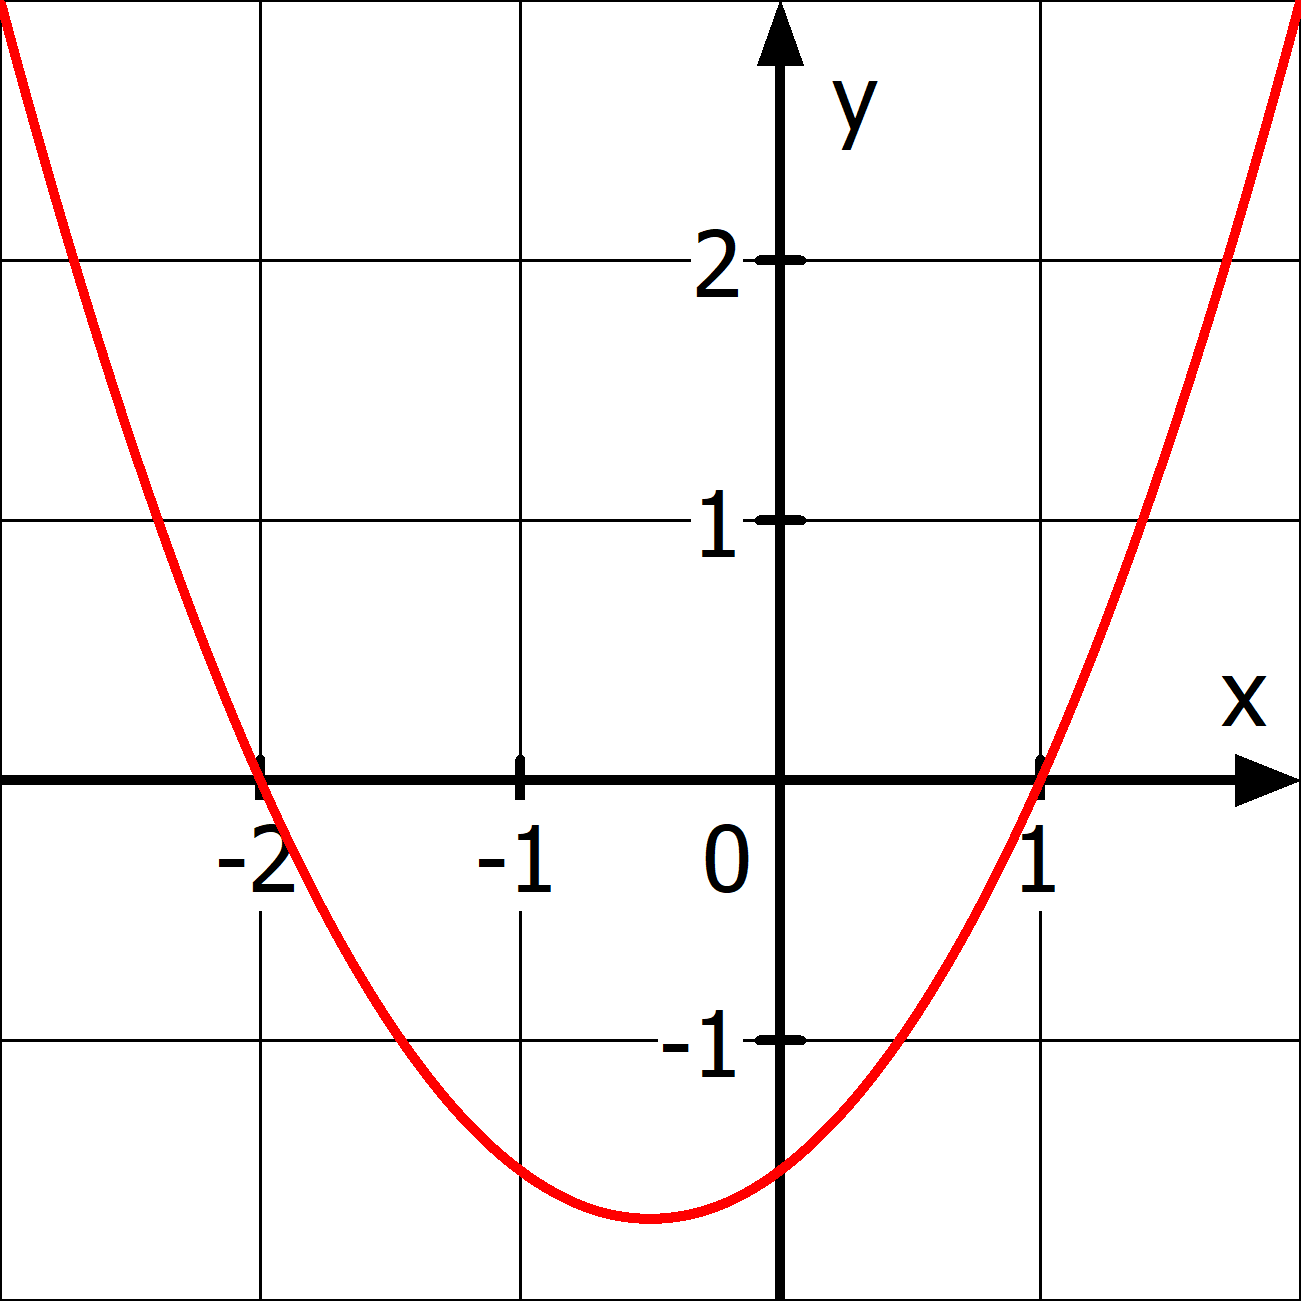
\includegraphics[width=\textwidth]{\ganzFkt/pics/produkt1.png}
	\end{minipage}}%
\end{minipage}

\bigskip

\begin{minipage}{\textwidth}
	\adjustbox{valign=t}{\begin{minipage}{0.5\textwidth-1ex}
		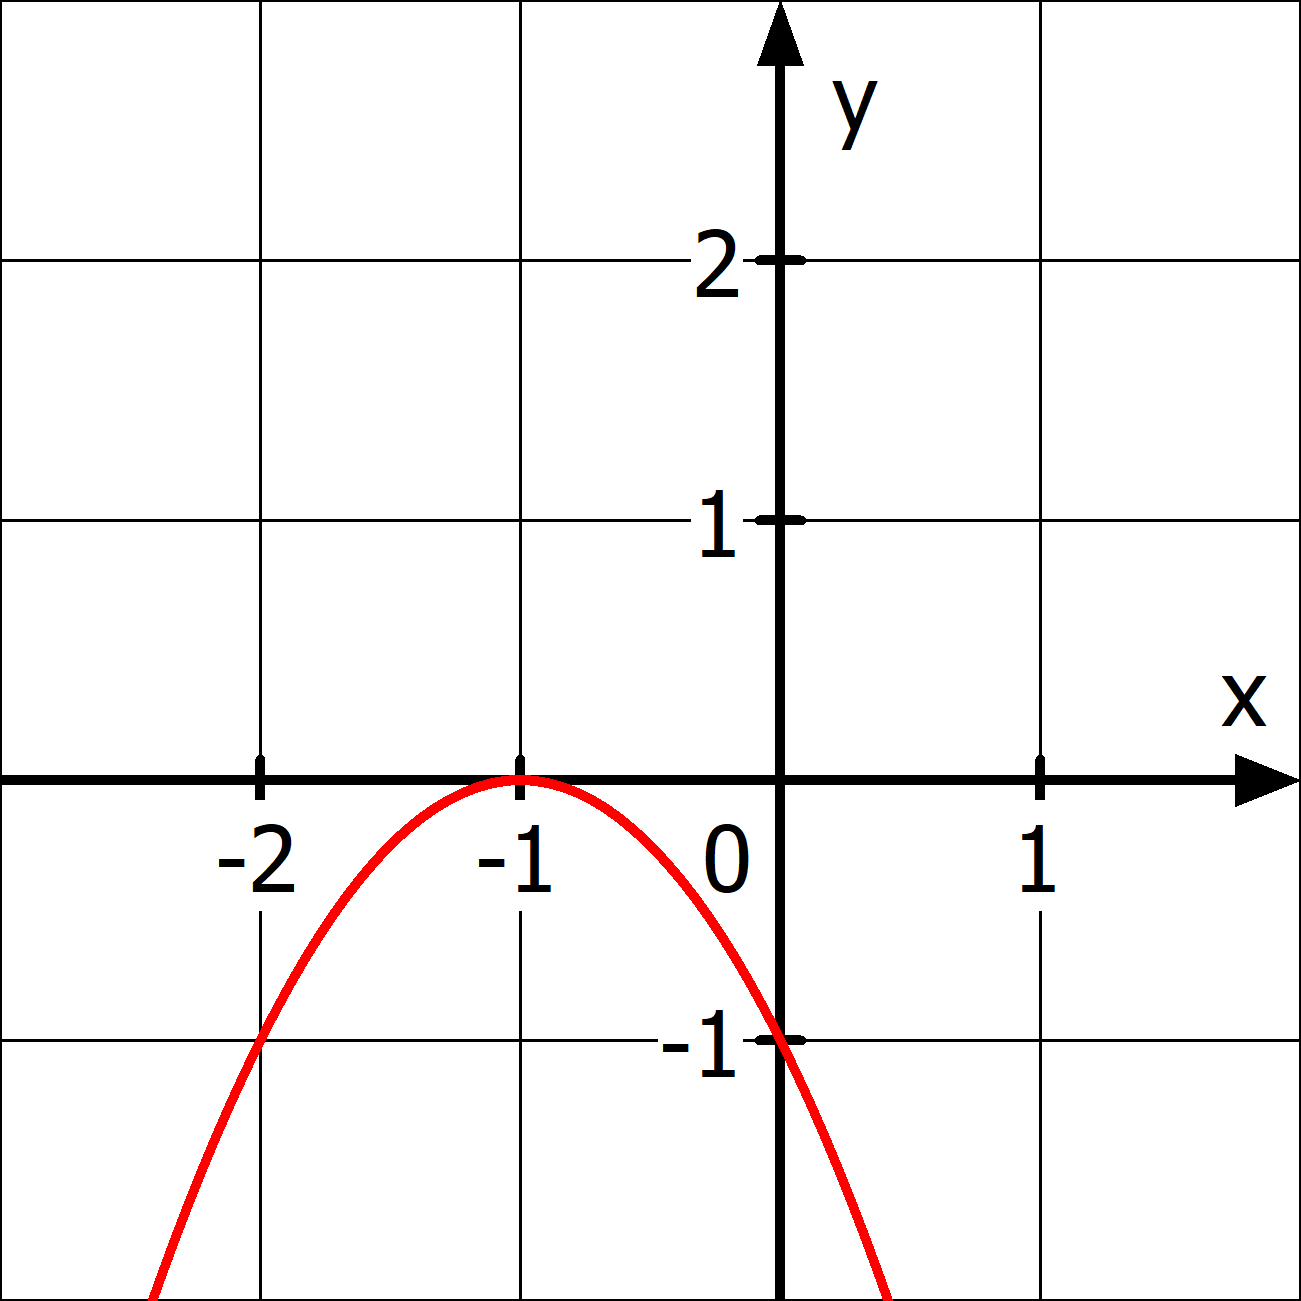
\includegraphics[width=\textwidth]{\ganzFkt/pics/produkt2.png}
	\end{minipage}}%
	\adjustbox{valign=t, padding =2ex 0ex 0ex 0ex}{{\color{loes}\begin{minipage}{0.5\textwidth-1ex}
			\textcolor{black}{Beispiel 2: \(f_2(x)=-0,5(x+2)^2x(x-1)^2\)}\\
			\begin{tabular}{rlcl}
				\multicolumn{2}{c}{NST}&VFH&Verlauf\\
				\midrule
				\(x_1\hspace{-0.3cm}\)&\(=-2\)&2&Parabelförmig\\
				\(x_2\hspace{-0.3cm}\)&\(=0\)&1&wie Gerade\\
				\(x_3\hspace{-0.3cm}\)&\(=1\)&3&Parabelförmig
			\end{tabular}
			Grad: \(2+1+2=2\)

			Leitkoeffizient \(a=-0,5\)

	\end{minipage}}}%
\end{minipage}

\bigskip

\begin{minipage}{\textwidth}
	\adjustbox{valign=t, padding =0ex 0ex 2ex 0ex}{{\color{loes}\begin{minipage}{0.5\textwidth-1ex}
			\textcolor{black}{Beispiel 3: \(f_3(x)=-x^3(x-2)\)}\\
			\begin{tabular}{rlcl}
				\multicolumn{2}{c}{NST}&VFH&Verlauf\\
				\midrule
				\(x_1\hspace{-0.3cm}\)&\(=0\)&1&S-förmig\\
				\(x_2\hspace{-0.3cm}\)&\(=2\)&2&wie Gerade
			\end{tabular}

			Grad: \(3+1=4\)

			Leitkoeffizient \(a=-1\)

	\end{minipage}}}%
	\adjustbox{valign=t}{\begin{minipage}{0.5\textwidth-1ex}
		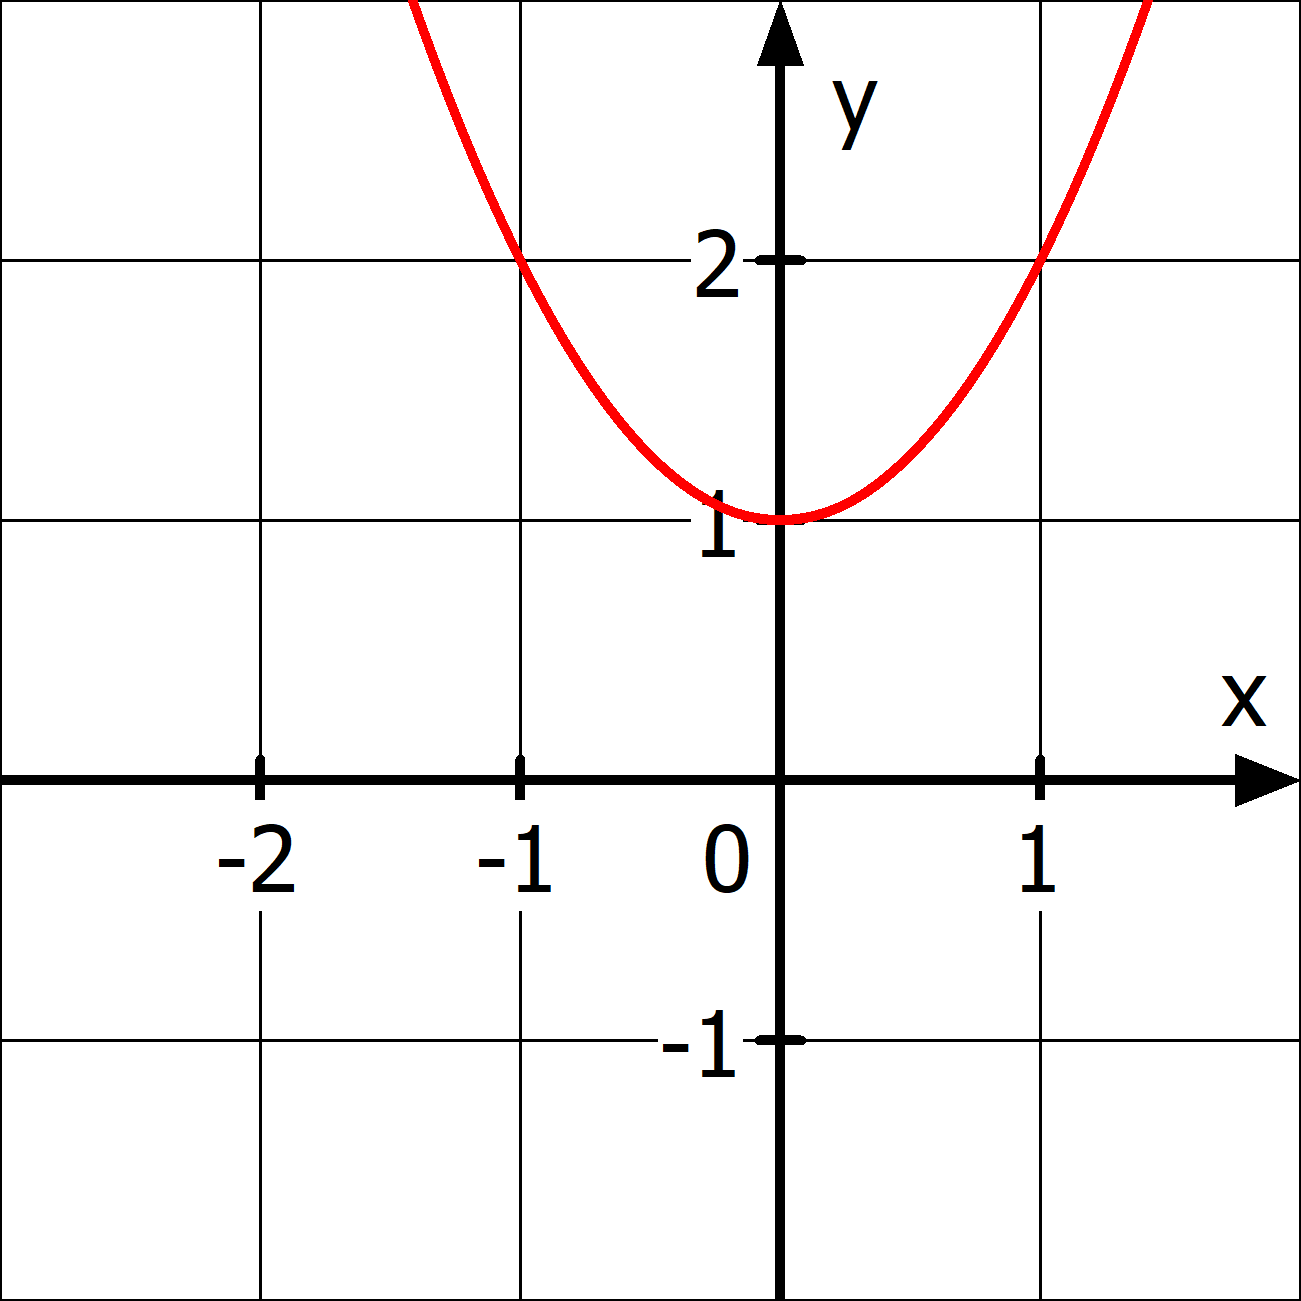
\includegraphics[width=\textwidth]{\ganzFkt/pics/produkt3.png}
	\end{minipage}}%
\end{minipage}
\newpage
%%%%%%%%%%%%%%%%%%%%%%%%%%%%%%%%%%%%%%%%%%%%%%%%%%%%%%%%%%%%%%%%%%%%%%%%%%%%%%%%%%%%%%%%%%%%%%%%%%%%%%%%%%%%%%%%%%%%%
Umgekehrt können wir ausgehend vom Schaubild die Funktionsgleichung aufstellen. Sind keine zusätzlichen Angaben zu den Vielfachheiten der Nullstellen gegeben, so probieren wir immer die kleinste mögliche Vielfachheit aus. Damit lässt sich dann die Funktionsgleichung mit Ausnahme des Leitkoeffizienten bestimmen. Dieser lässt sich mit einer Punktprobe berechnen.

\bigskip

\begin{minipage}{\textwidth}
	\adjustbox{valign=t, padding =0ex 0ex 2ex 0ex}{{\color{loes}\begin{minipage}{0.5\textwidth-1ex}
			\textcolor{black}{Beispiel 1:}\\
			\begin{tabular}{rllc}
				\multicolumn{2}{c}{NST}&Verlauf&VFH\\
				\midrule
				\(x_1\hspace{-0.3cm}\)&\(=-1\)&Parabelförmig&gerade\\
				\(x_2\hspace{-0.3cm}\)&\(=1\)&wie Gerade&1\\
				\(x_3\hspace{-0.3cm}\)&\(=2\)&wie Gerade&1
			\end{tabular}\\
			Nehmen wir für die erste Nullstelle die kleinste mögliche Vielfachheit, also 2, so ergibt sich\\
			\(f_1(x)=a\left(x+1\right)^2 \left(x-1\right) \left(x-2\right) \)\\
			Eine Punktprobe mit \(P(0\vert-1)\), also \(f_1(0)=-1\) ergibt \(a=-0,5\) und damit\\
			\(f_1(x)=-0,5\left(x+1\right)^2 \left(x-1\right) \left(x-2\right) \)
	\end{minipage}}}%
	\adjustbox{valign=t}{\begin{minipage}{0.5\textwidth-1ex}
		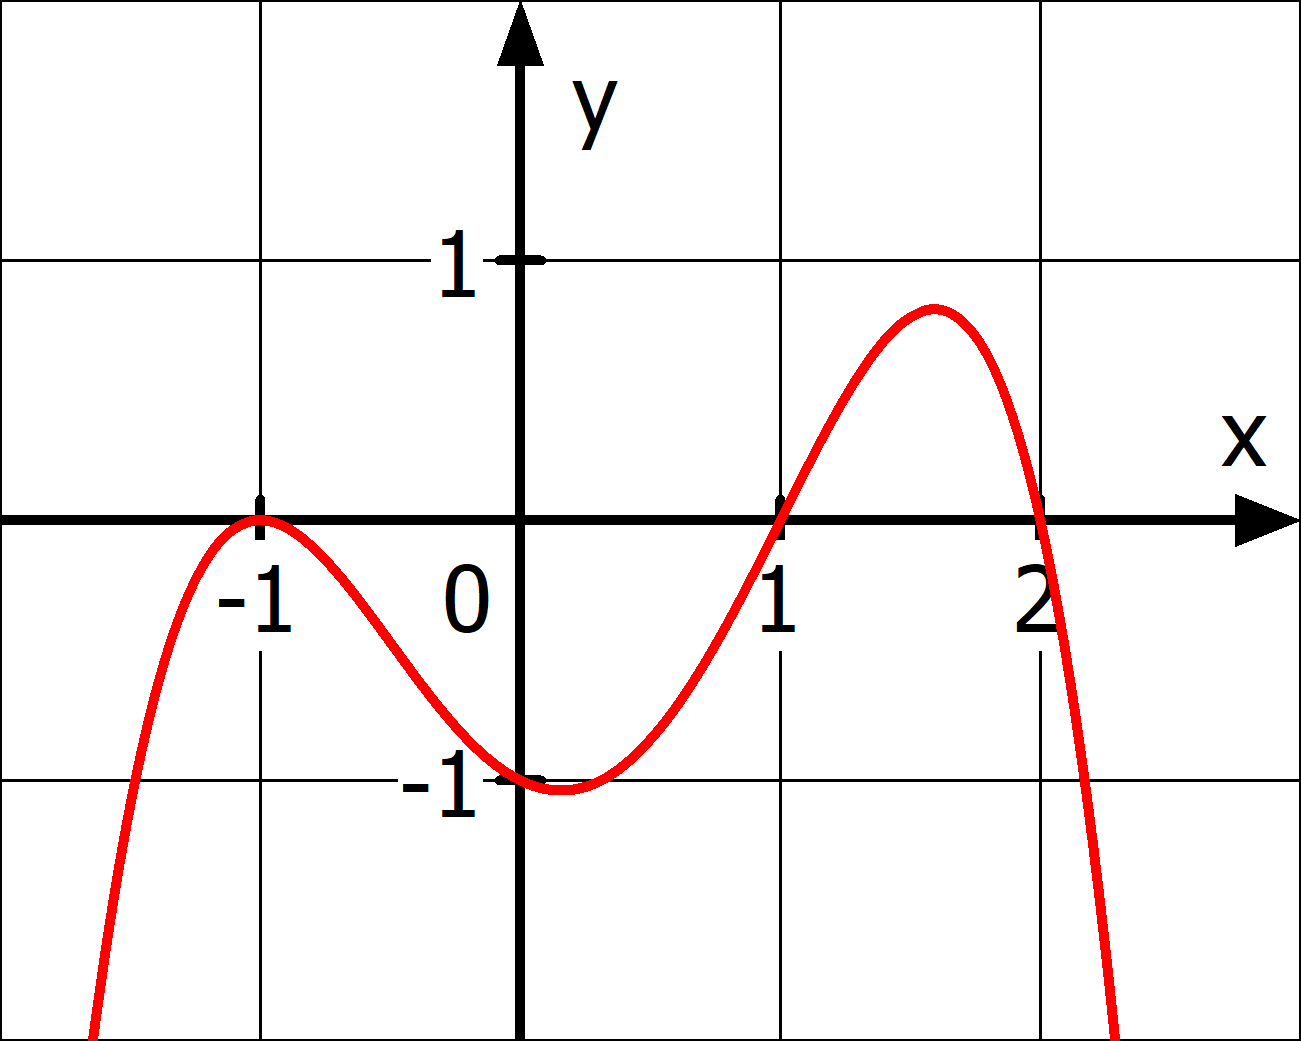
\includegraphics[width=\textwidth]{\ganzFkt/pics/produkt4.png}
	\end{minipage}}%
\end{minipage}

\bigskip

\begin{minipage}{\textwidth}
	\adjustbox{valign=t}{\begin{minipage}{0.5\textwidth-1ex}
		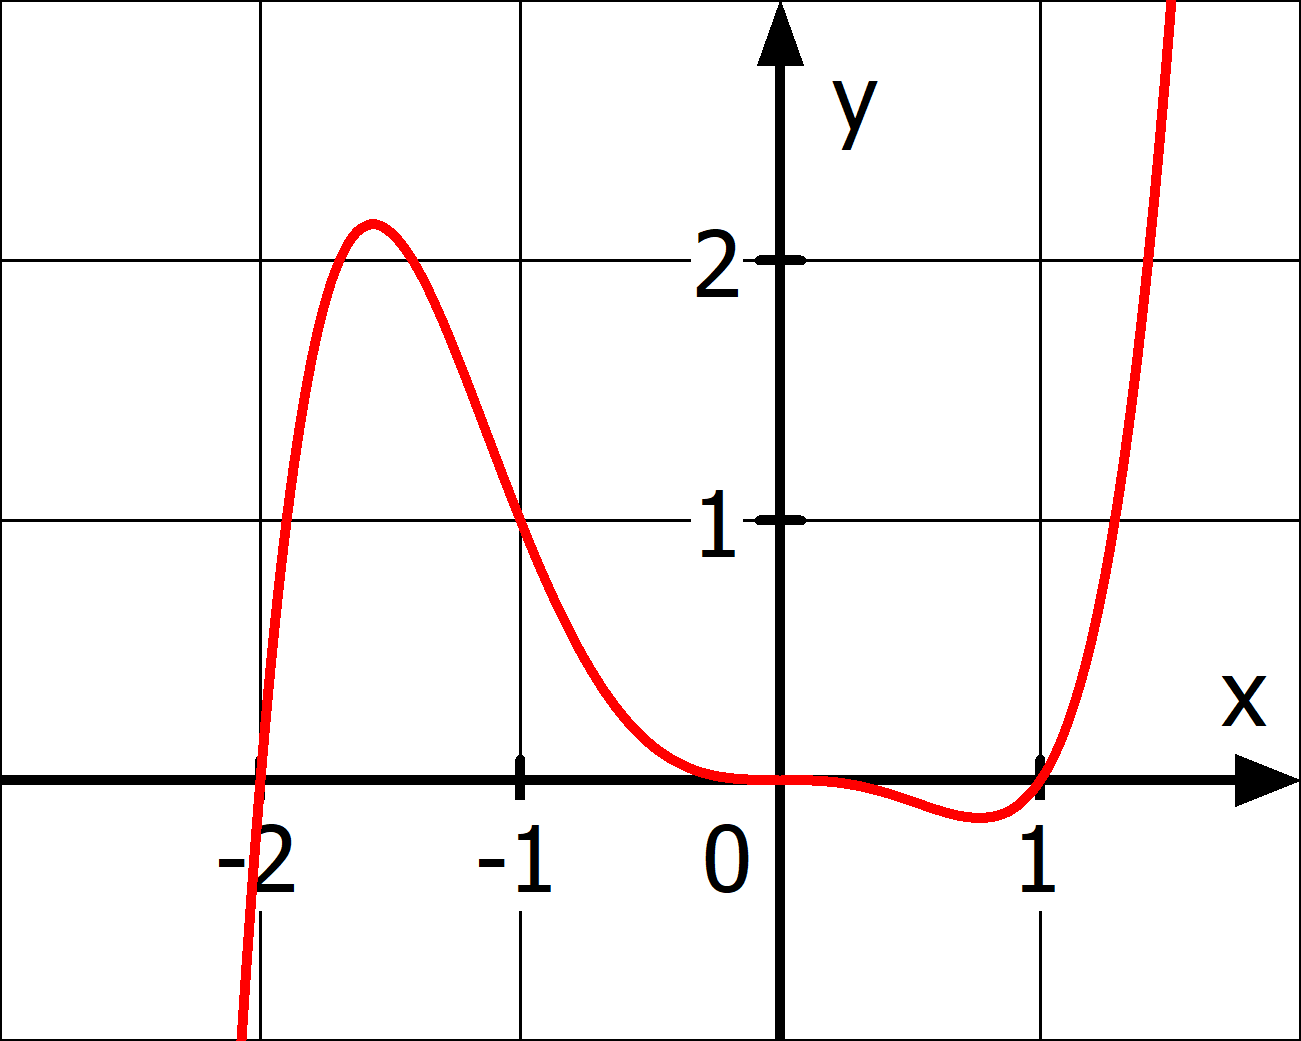
\includegraphics[width=\textwidth]{\ganzFkt/pics/produkt5.png}
	\end{minipage}}%
	\adjustbox{valign=t, padding =2ex 0ex 0ex 0ex}{{\color{loes}\begin{minipage}{0.5\textwidth-1ex}
			\textcolor{black}{Beispiel 2:}

			\begin{tabular}{rllc}
				\multicolumn{2}{c}{NST}&Verlauf&VFH\\
				\midrule
				\(x_1\hspace{-0.3cm}\)&\(=-2\)&wie Gerade&1\\
				\(x_2\hspace{-0.3cm}\)&\(=0\)&S-förmig&\(3,\ 5,\ \dots\)\\
				\(x_3\hspace{-0.3cm}\)&\(=1\)&wie Gerade&1
			\end{tabular}\\
			Nehmen wir für die zweite Nullstelle die kleinste mögliche Vielfachheit, also 3, so ergibt sich

			\(f_2(x)=a\left(x+2\right)x^3 \left(x-1\right) \)

			Eine Punktprobe mit \(P(-1\vert 1)\), also \(f_1(-1)=1\) ergibt \(a=0,5\) und damit

			\(f_2(x)=0,5\left(x+2\right)x^3 \left(x-1\right) \)
	\end{minipage}}}%
\end{minipage}

\bigskip

\begin{minipage}{\textwidth}
	\adjustbox{valign=t, padding =0ex 0ex 2ex 0ex}{{\color{loes}\begin{minipage}{0.5\textwidth-1ex}
			\textcolor{black}{Beispiel 3:}

			\begin{tabular}{rllc}
				\multicolumn{2}{c}{NST}&Verlauf&VFH\\
				\midrule
				\(x_1\hspace{-0.3cm}\)&\(=0\)&wie Gerade&1\\
				\(x_2\hspace{-0.3cm}\)&\(=2\)&wie Gerade&1\\
				\(x_3\hspace{-0.3cm}\)&\(=3\)&wie Gerade&1
			\end{tabular}

			Es ergibt sich aus den Nullstellen:

			\(f_3(x)=ax \left(x-2\right) \left(x-3\right) \)

			Eine Punktprobe mit \(P(1\vert-2)\), also \(f_1(1)=-2\) ergibt \(a=-1\) und damit

			\(f_3(x)=-x \left(x-2\right) \left(x-3\right) \)
	\end{minipage}}}%
	\adjustbox{valign=t}{\begin{minipage}{0.5\textwidth-1ex}
		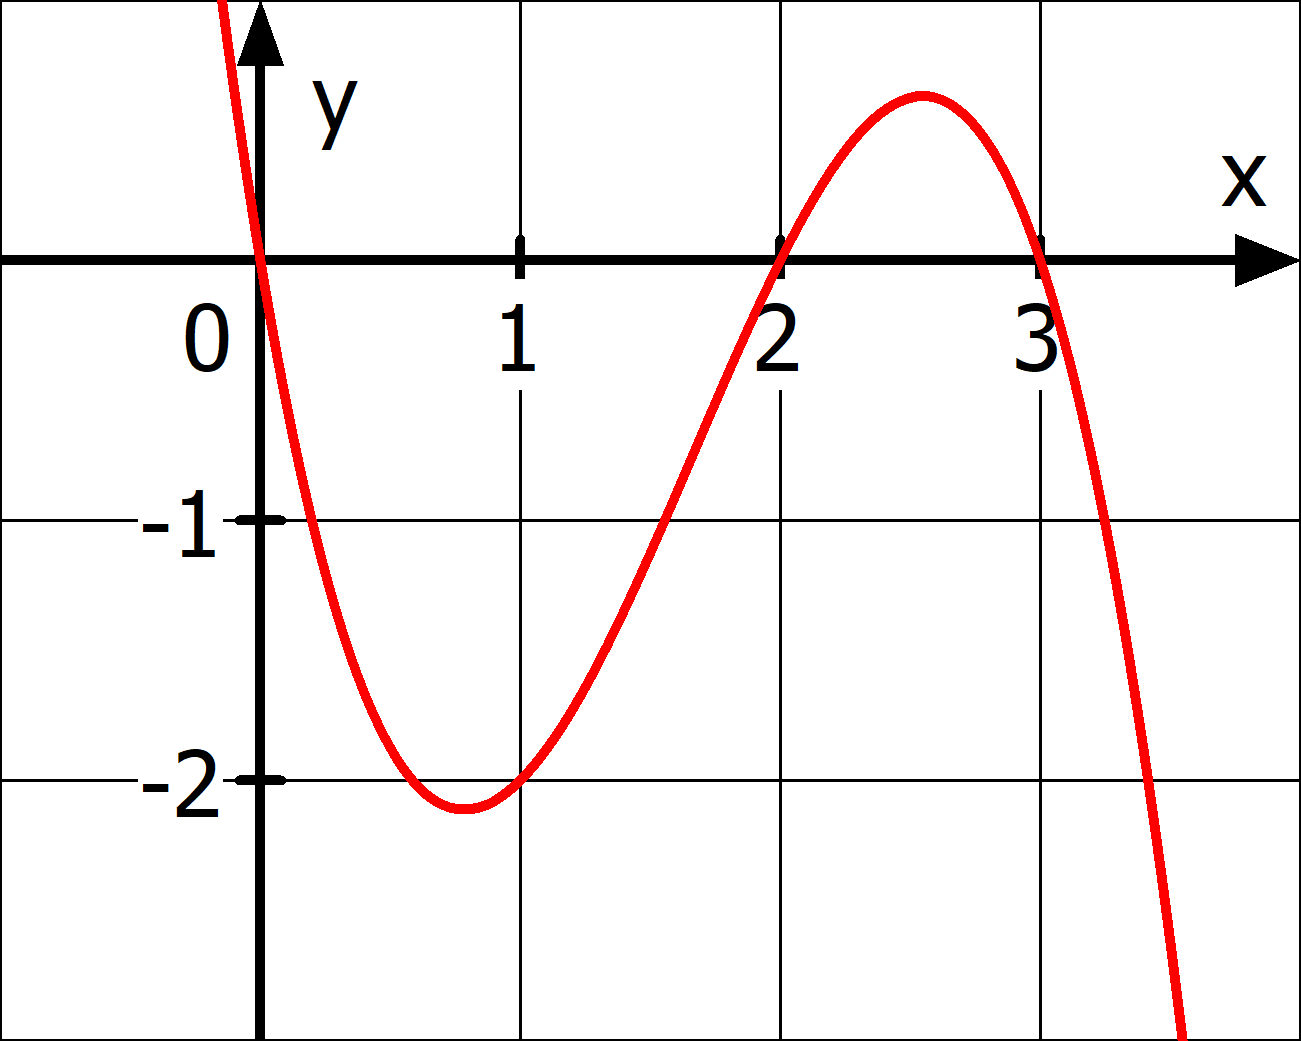
\includegraphics[width=\textwidth]{\ganzFkt/pics/produkt6.png}
	\end{minipage}}%
\end{minipage}
\newpage
%%%%%%%%%%%%%%%%%%%%%%%%%%%%%%%%%%%%%%%%%%%%%%%%%%%%%%%%%%%%%%%%%%%%%%%%%%%%%%%%%%%%%%%%%%%%%%%%%%%%%%%%%%%%%%%%%%%%%
\begin{Exercise}[title={Skizziere das Schaubild}, label=ganzProduktA1]\\
	\begin{minipage}{\textwidth}
		\begin{minipage}{0.5\textwidth}
			\begin{enumerate}[label=\alph*)]
				\item \(f(x)=0,1\left(x+3\right)^2\left(x+1\right)\left(x-1\right)^3\)
				\item \(g(x)=-\frac{1}{5}\left(x+4\right) \left(x+3\right) \left(x+1\right) x^2 \)
				\item \(h(x)=-\left(x+1\right)^3 \left(x-1\right)^2 \left(x-2\right)\)
				\item \(i(x)=\frac{1}{3}x^2\left(x+1\right) \left( x-2\right) \left( x-3\right) ^2\)
			\end{enumerate}
		\end{minipage}%
		\begin{minipage}{0.5\textwidth}
			\begin{enumerate}[label=\alph*)]
				\setcounter{enumi}{4}
				\item \(j(x)=\frac{1}{5}\left( x+2\right) x\left( x-2\right) ^2\)
				\item \(k(x)=-x^3\left( x-2\right) ^2\)
				\item \(l(x)=\frac{1}{10}\left( x+4\right) ^2 x^2\)
				\item \(m(x)=-\frac{3}{35}\left( x+5\right) \left( x+4\right) ^2\left( x+2\right) x\)
			\end{enumerate}
		\end{minipage}%
	\end{minipage}
\end{Exercise}
\begin{Exercise}[title={Stelle die Funktionsgleichung auf. Verwende jeweils die kleinstmögliche Vielfachheit.}, label=ganzProduktA2]\\
	\begin{minipage}{\textwidth}
		\begin{minipage}{0.5\textwidth}
			\begin{enumerate}[label=\alph*)]
				\item \begin{minipage}[t]{0.8\textwidth}\vspace{-0.5\baselineskip}
					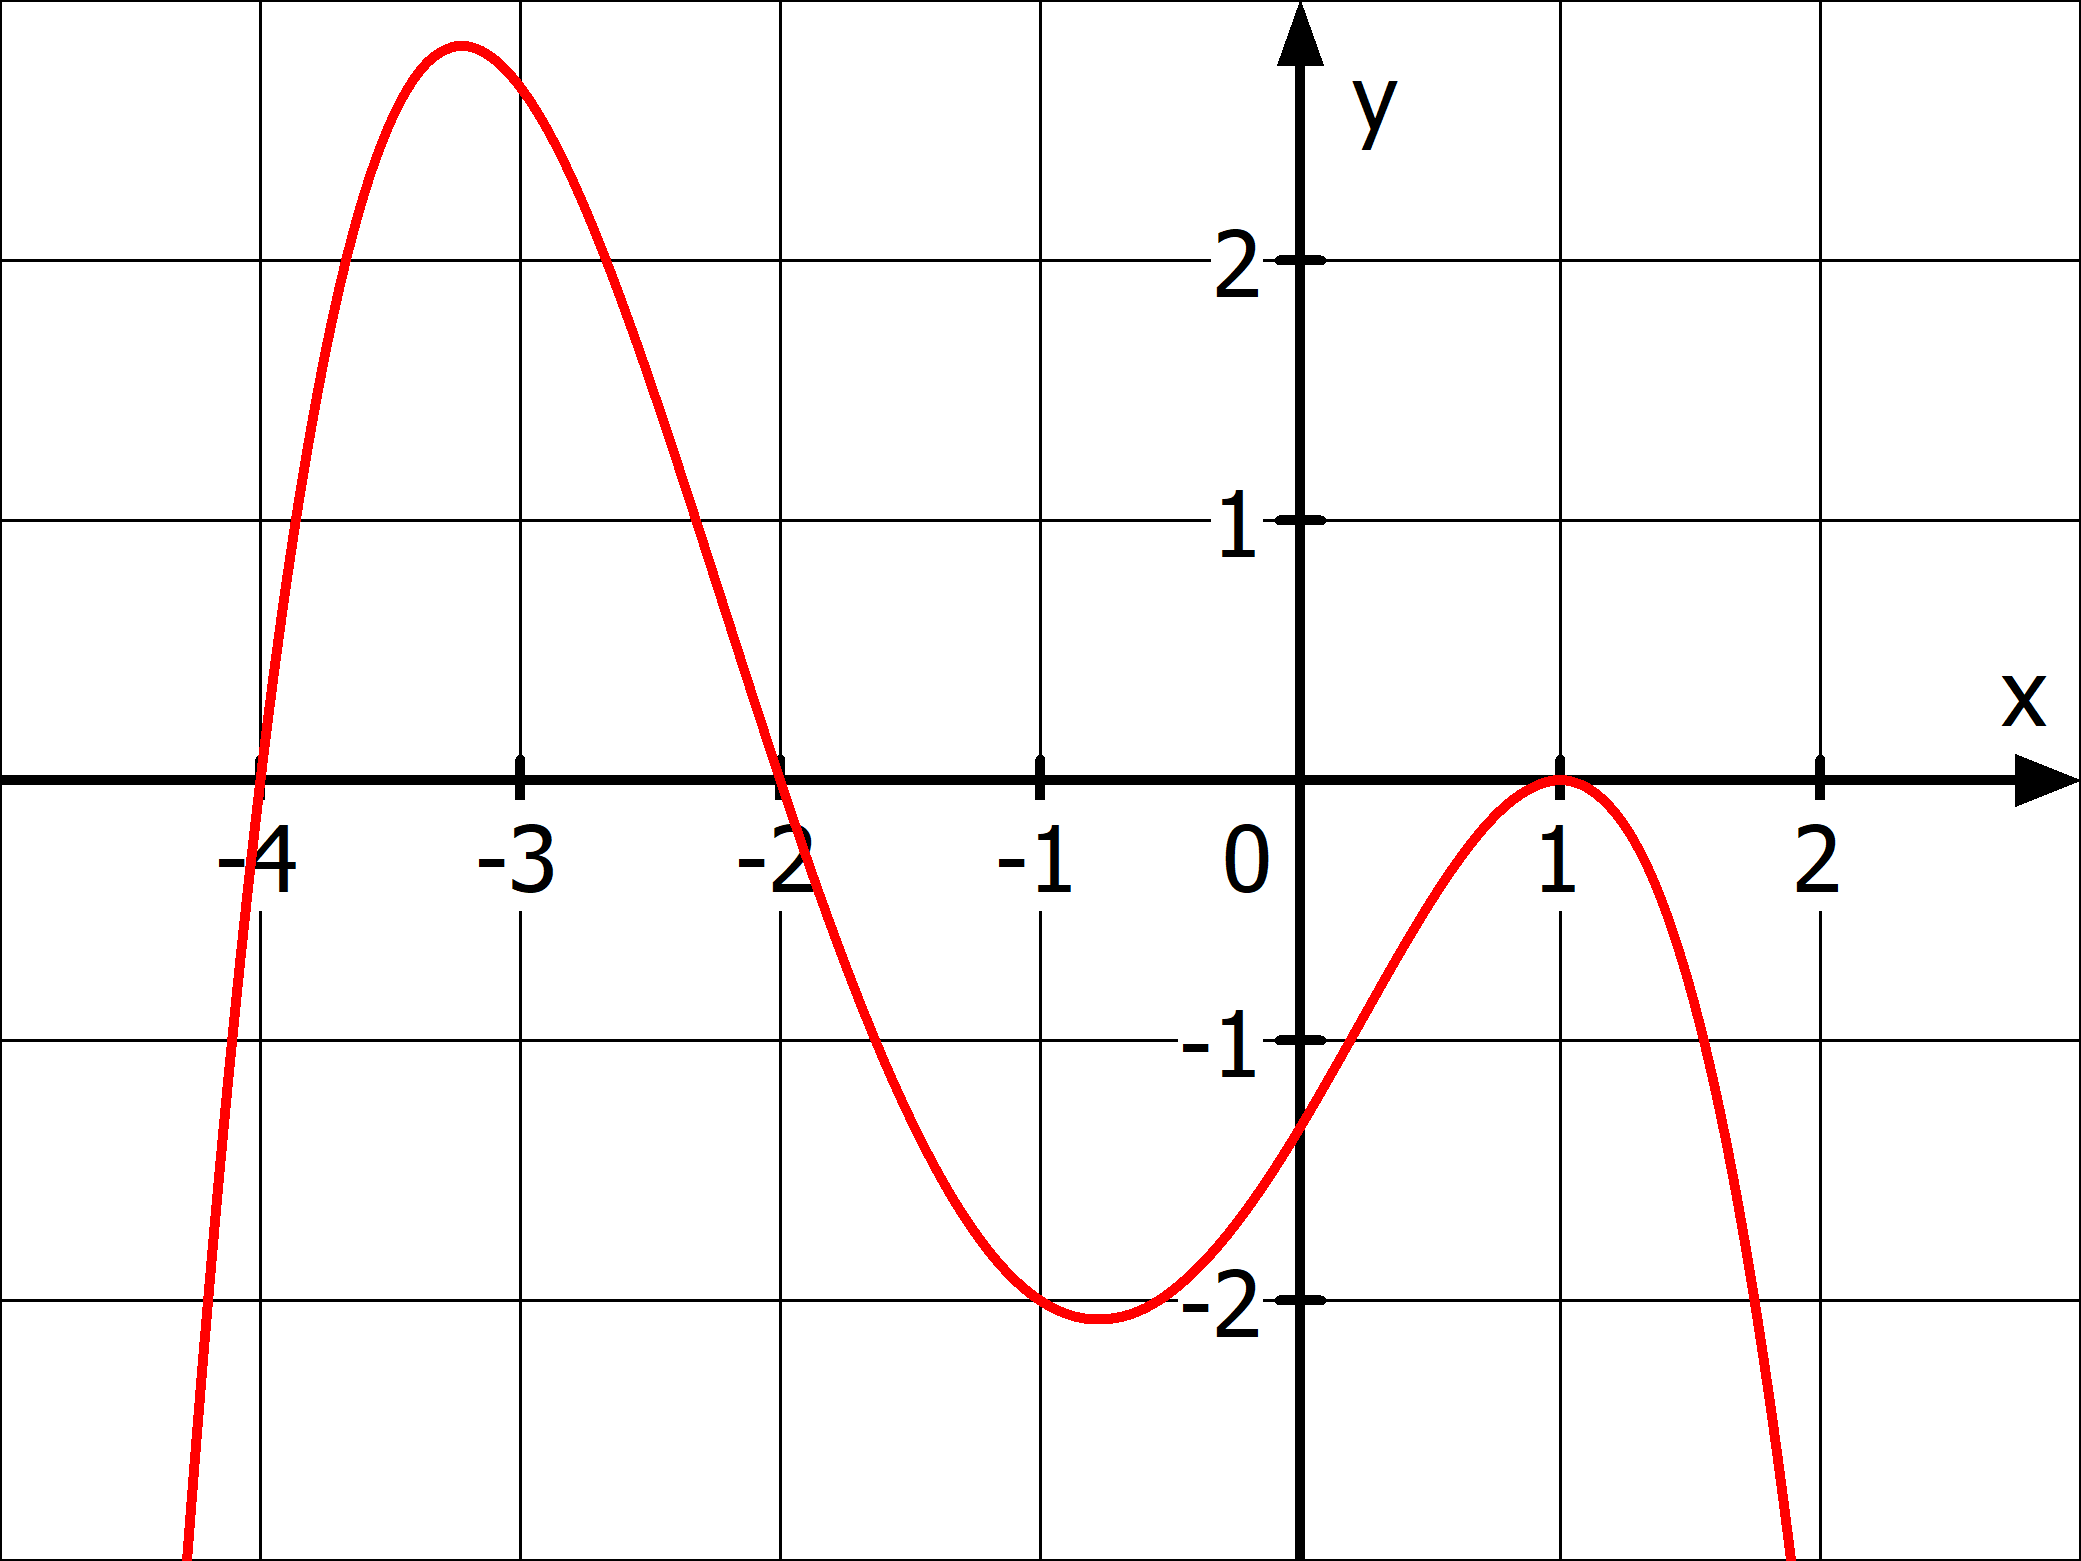
\includegraphics[width=\textwidth]{\ganzFkt/pics/produktA2_1.png}%
				\end{minipage}%

                \bigskip

				\item \begin{minipage}[t]{0.8\textwidth}\vspace{-0.5\baselineskip}
					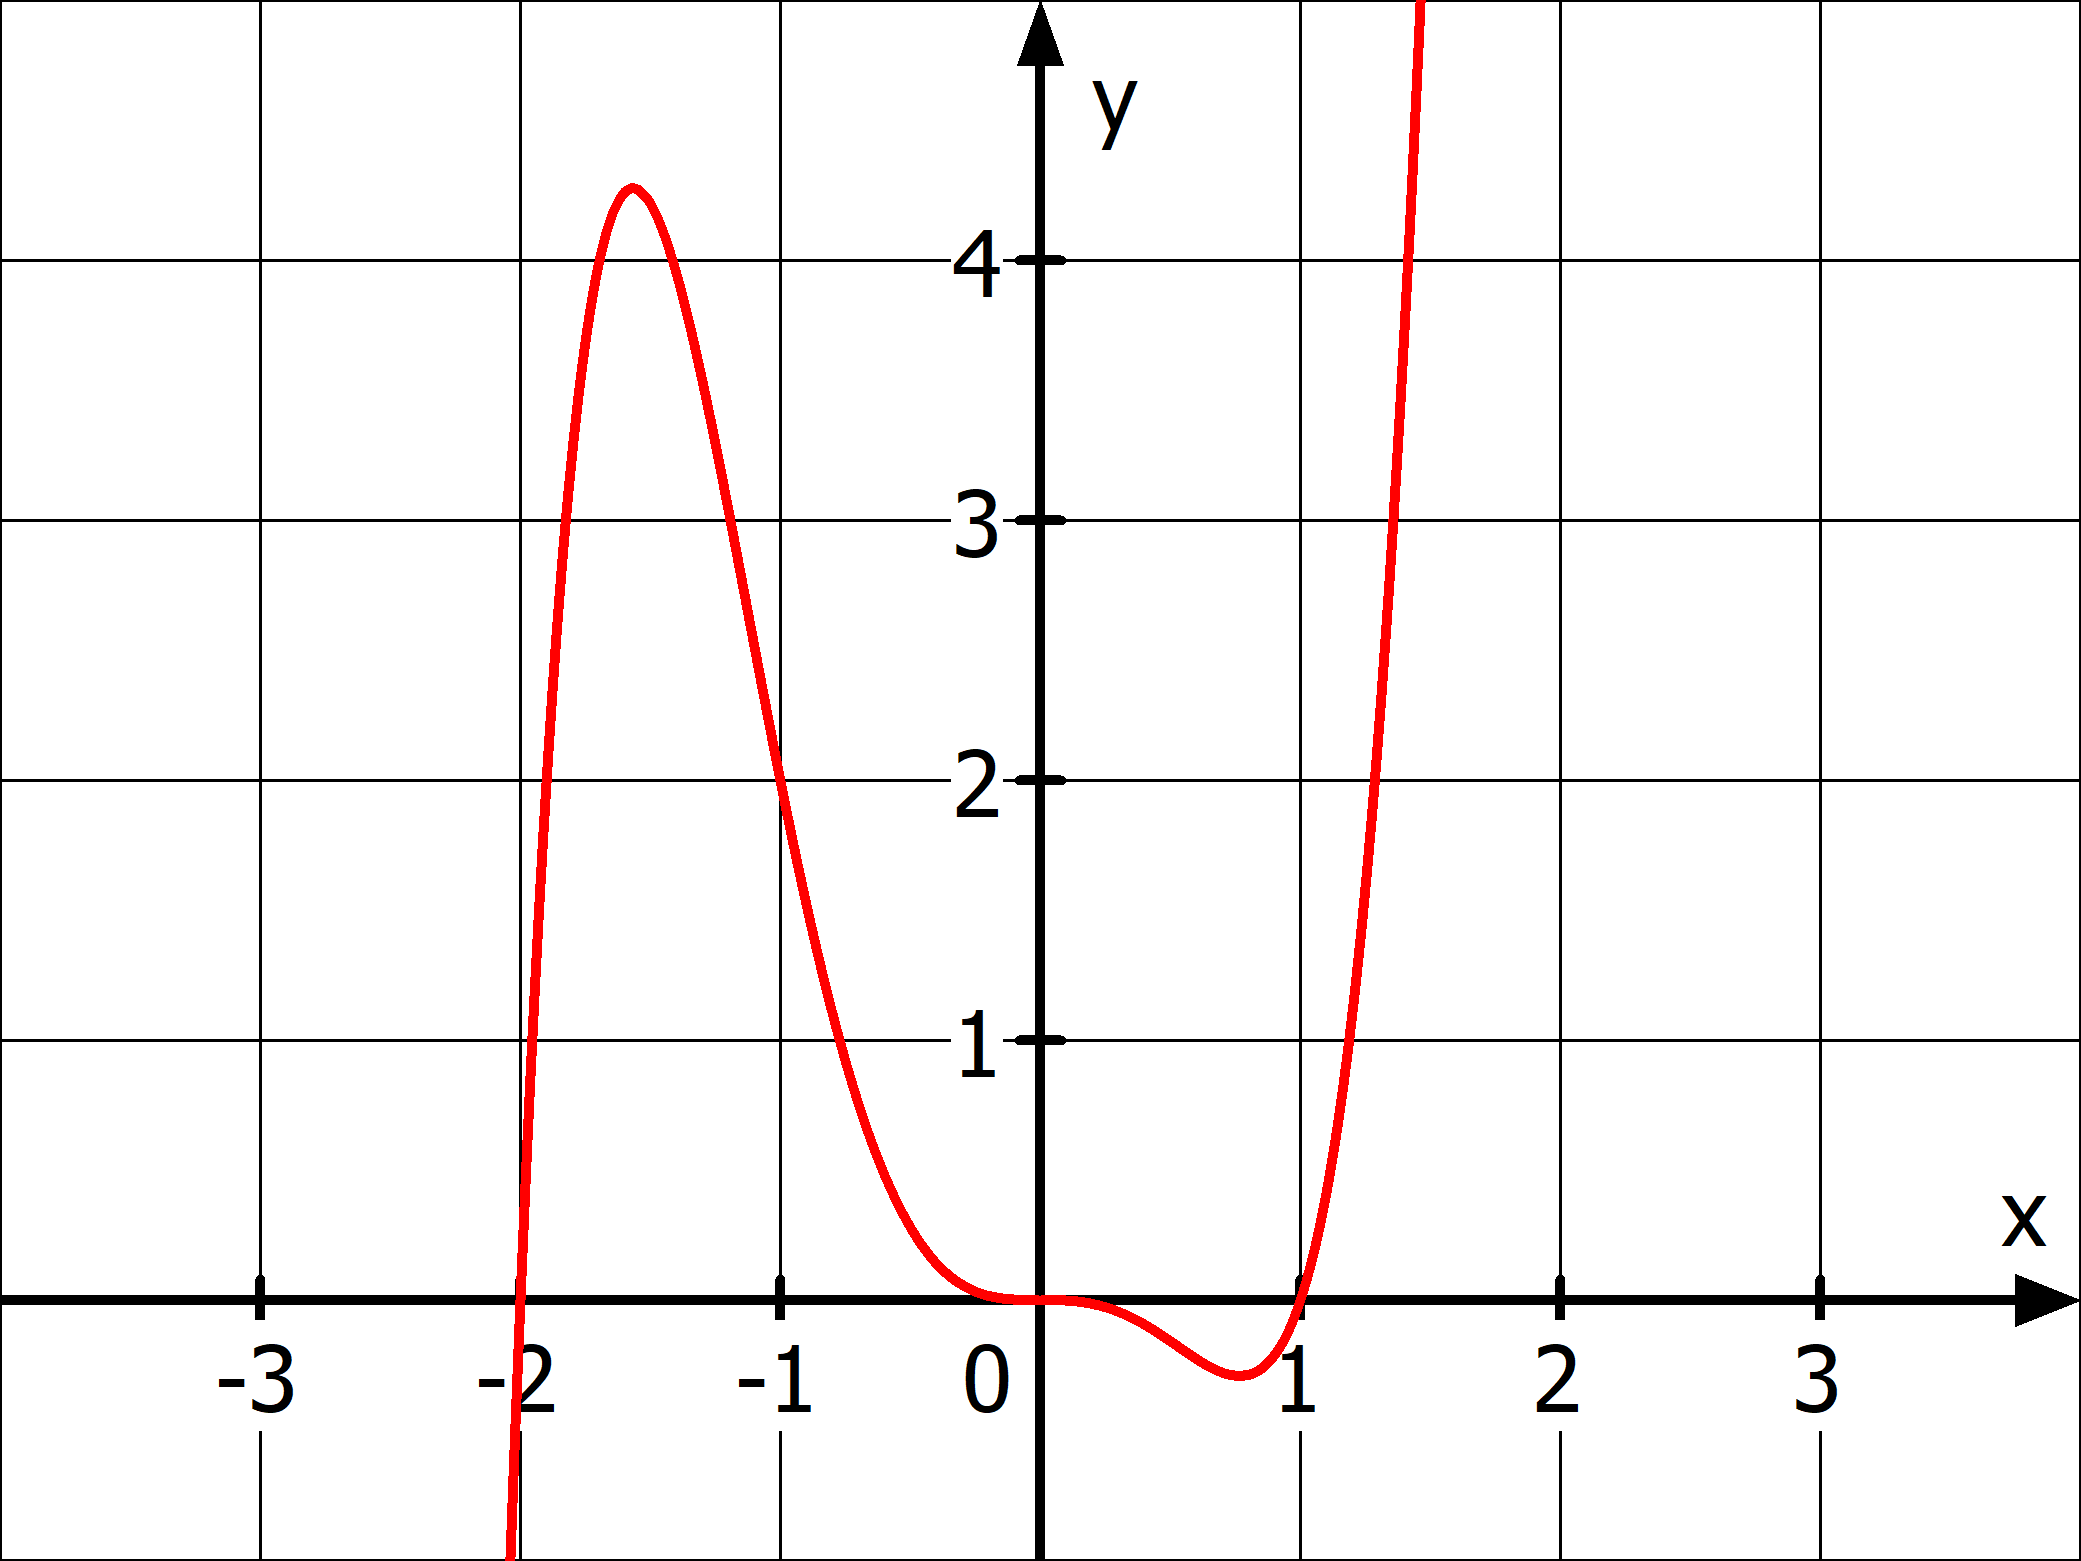
\includegraphics[width=\textwidth]{\ganzFkt/pics/produktA2_2.png}%
				\end{minipage}%

                \bigskip

				\item \begin{minipage}[t]{0.8\textwidth}\vspace{-0.5\baselineskip}
					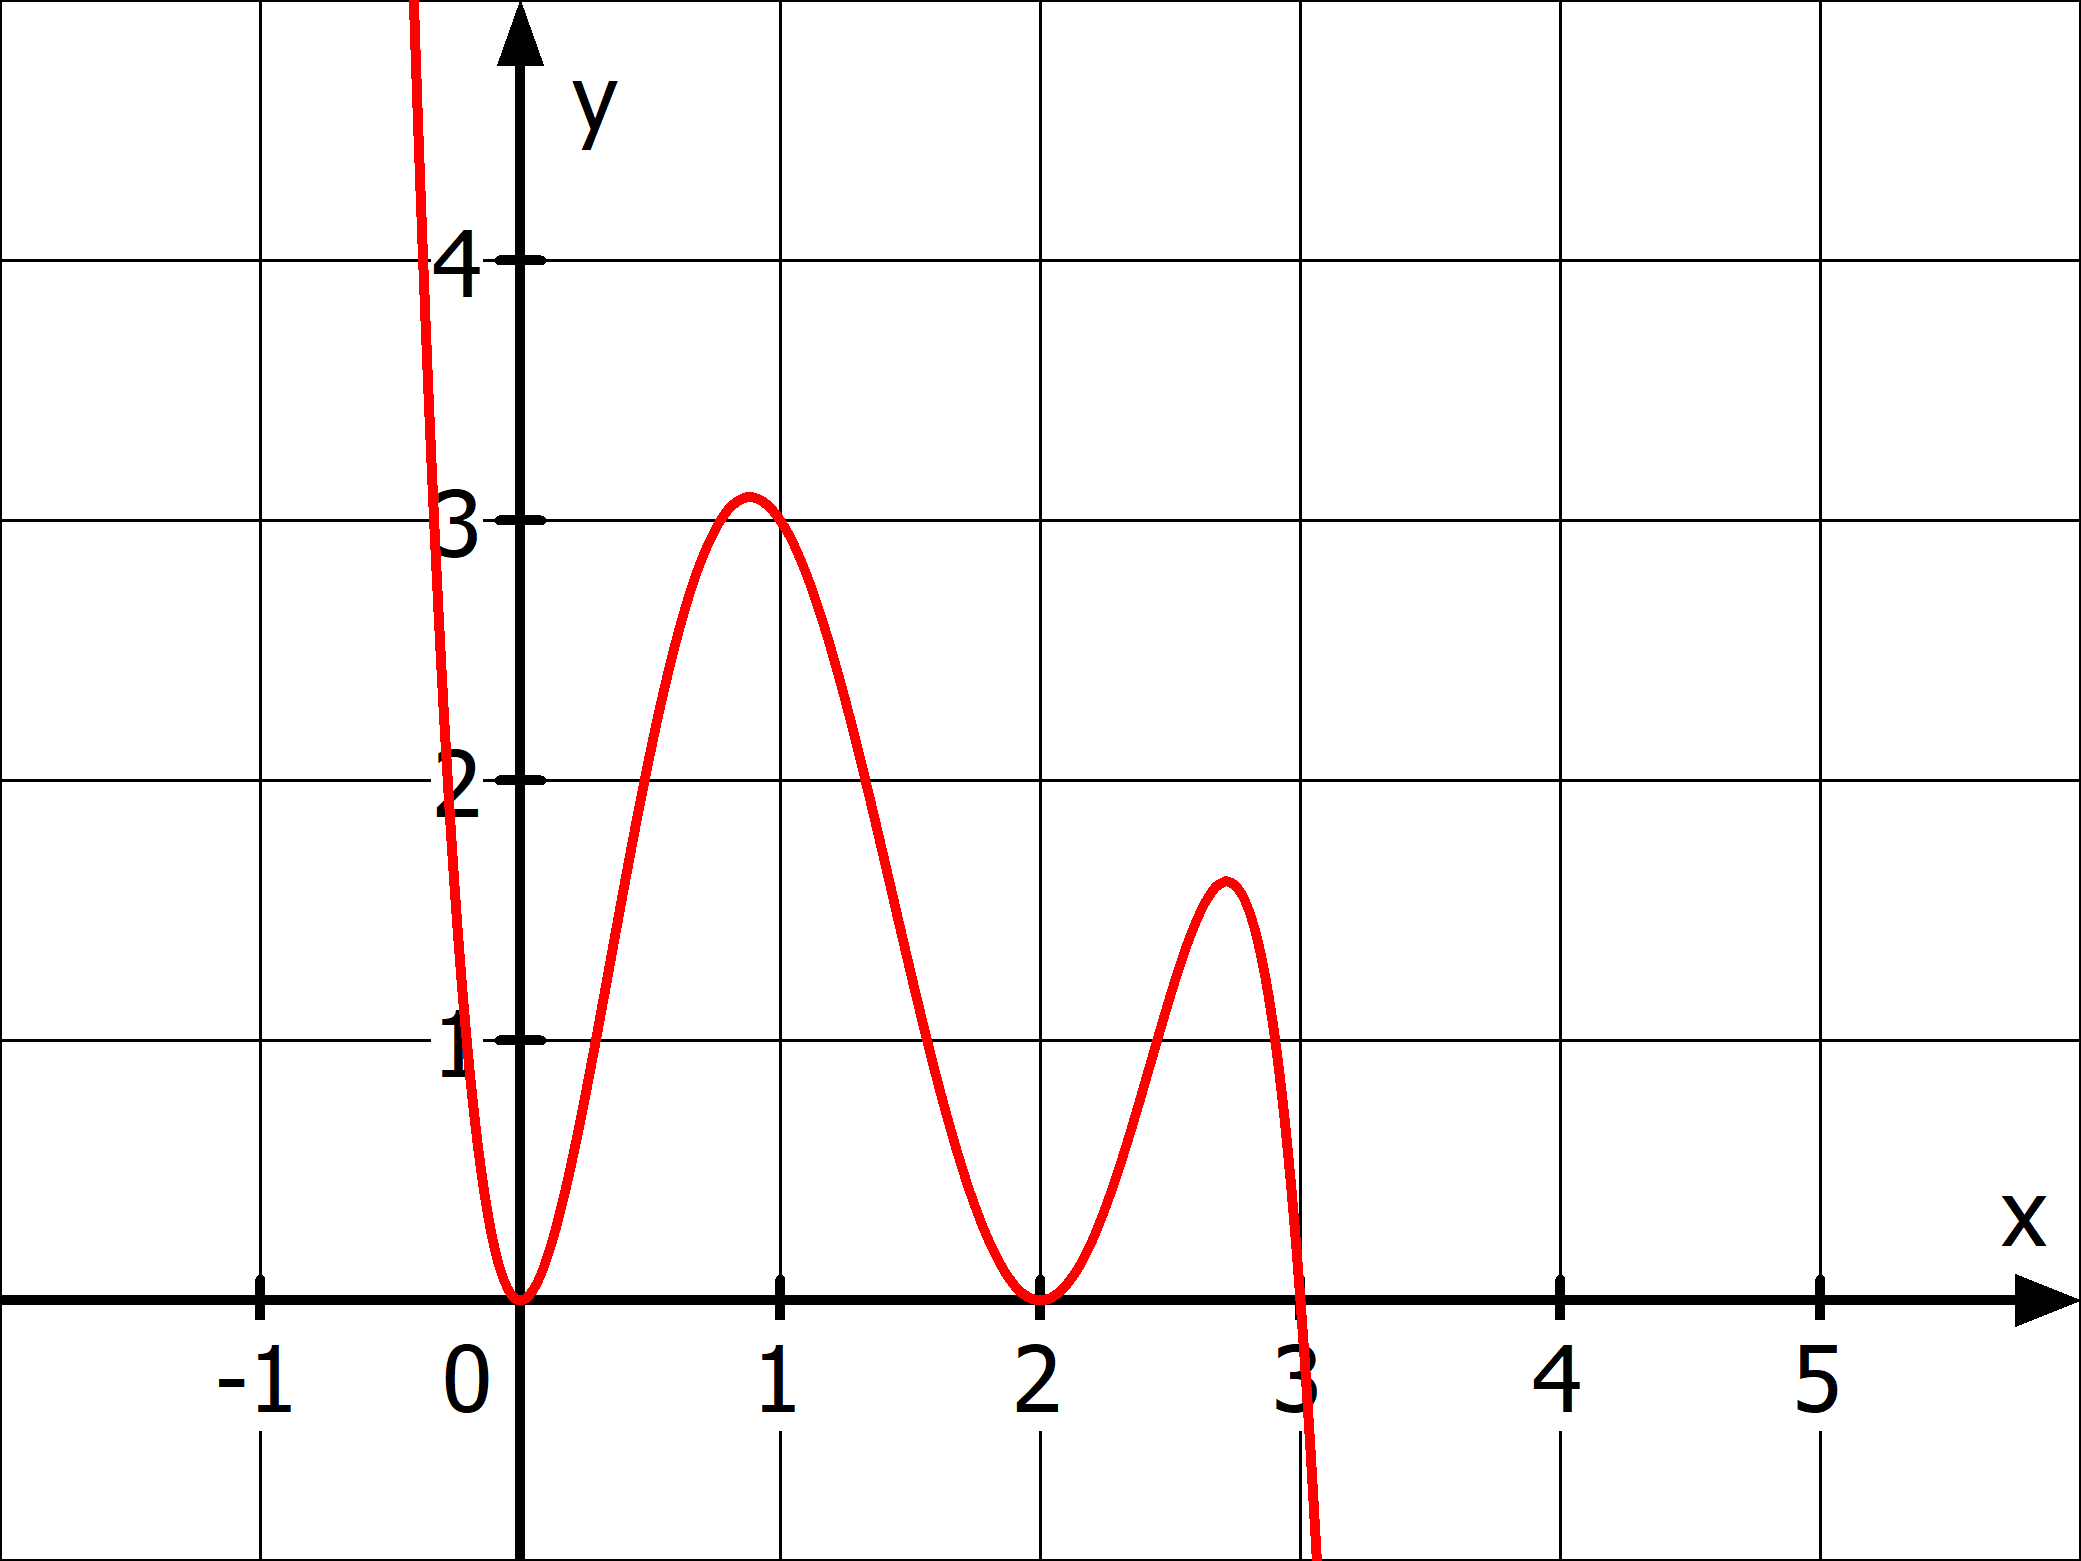
\includegraphics[width=\textwidth]{\ganzFkt/pics/produktA2_3.png}%
				\end{minipage}%
			\end{enumerate}%
		\end{minipage}%
		\begin{minipage}{0.5\textwidth}
			\begin{enumerate}[label=\alph*)]
				\setcounter{enumi}{3}
				\item \begin{minipage}[t]{0.8\textwidth}\vspace{-0.5\baselineskip}
					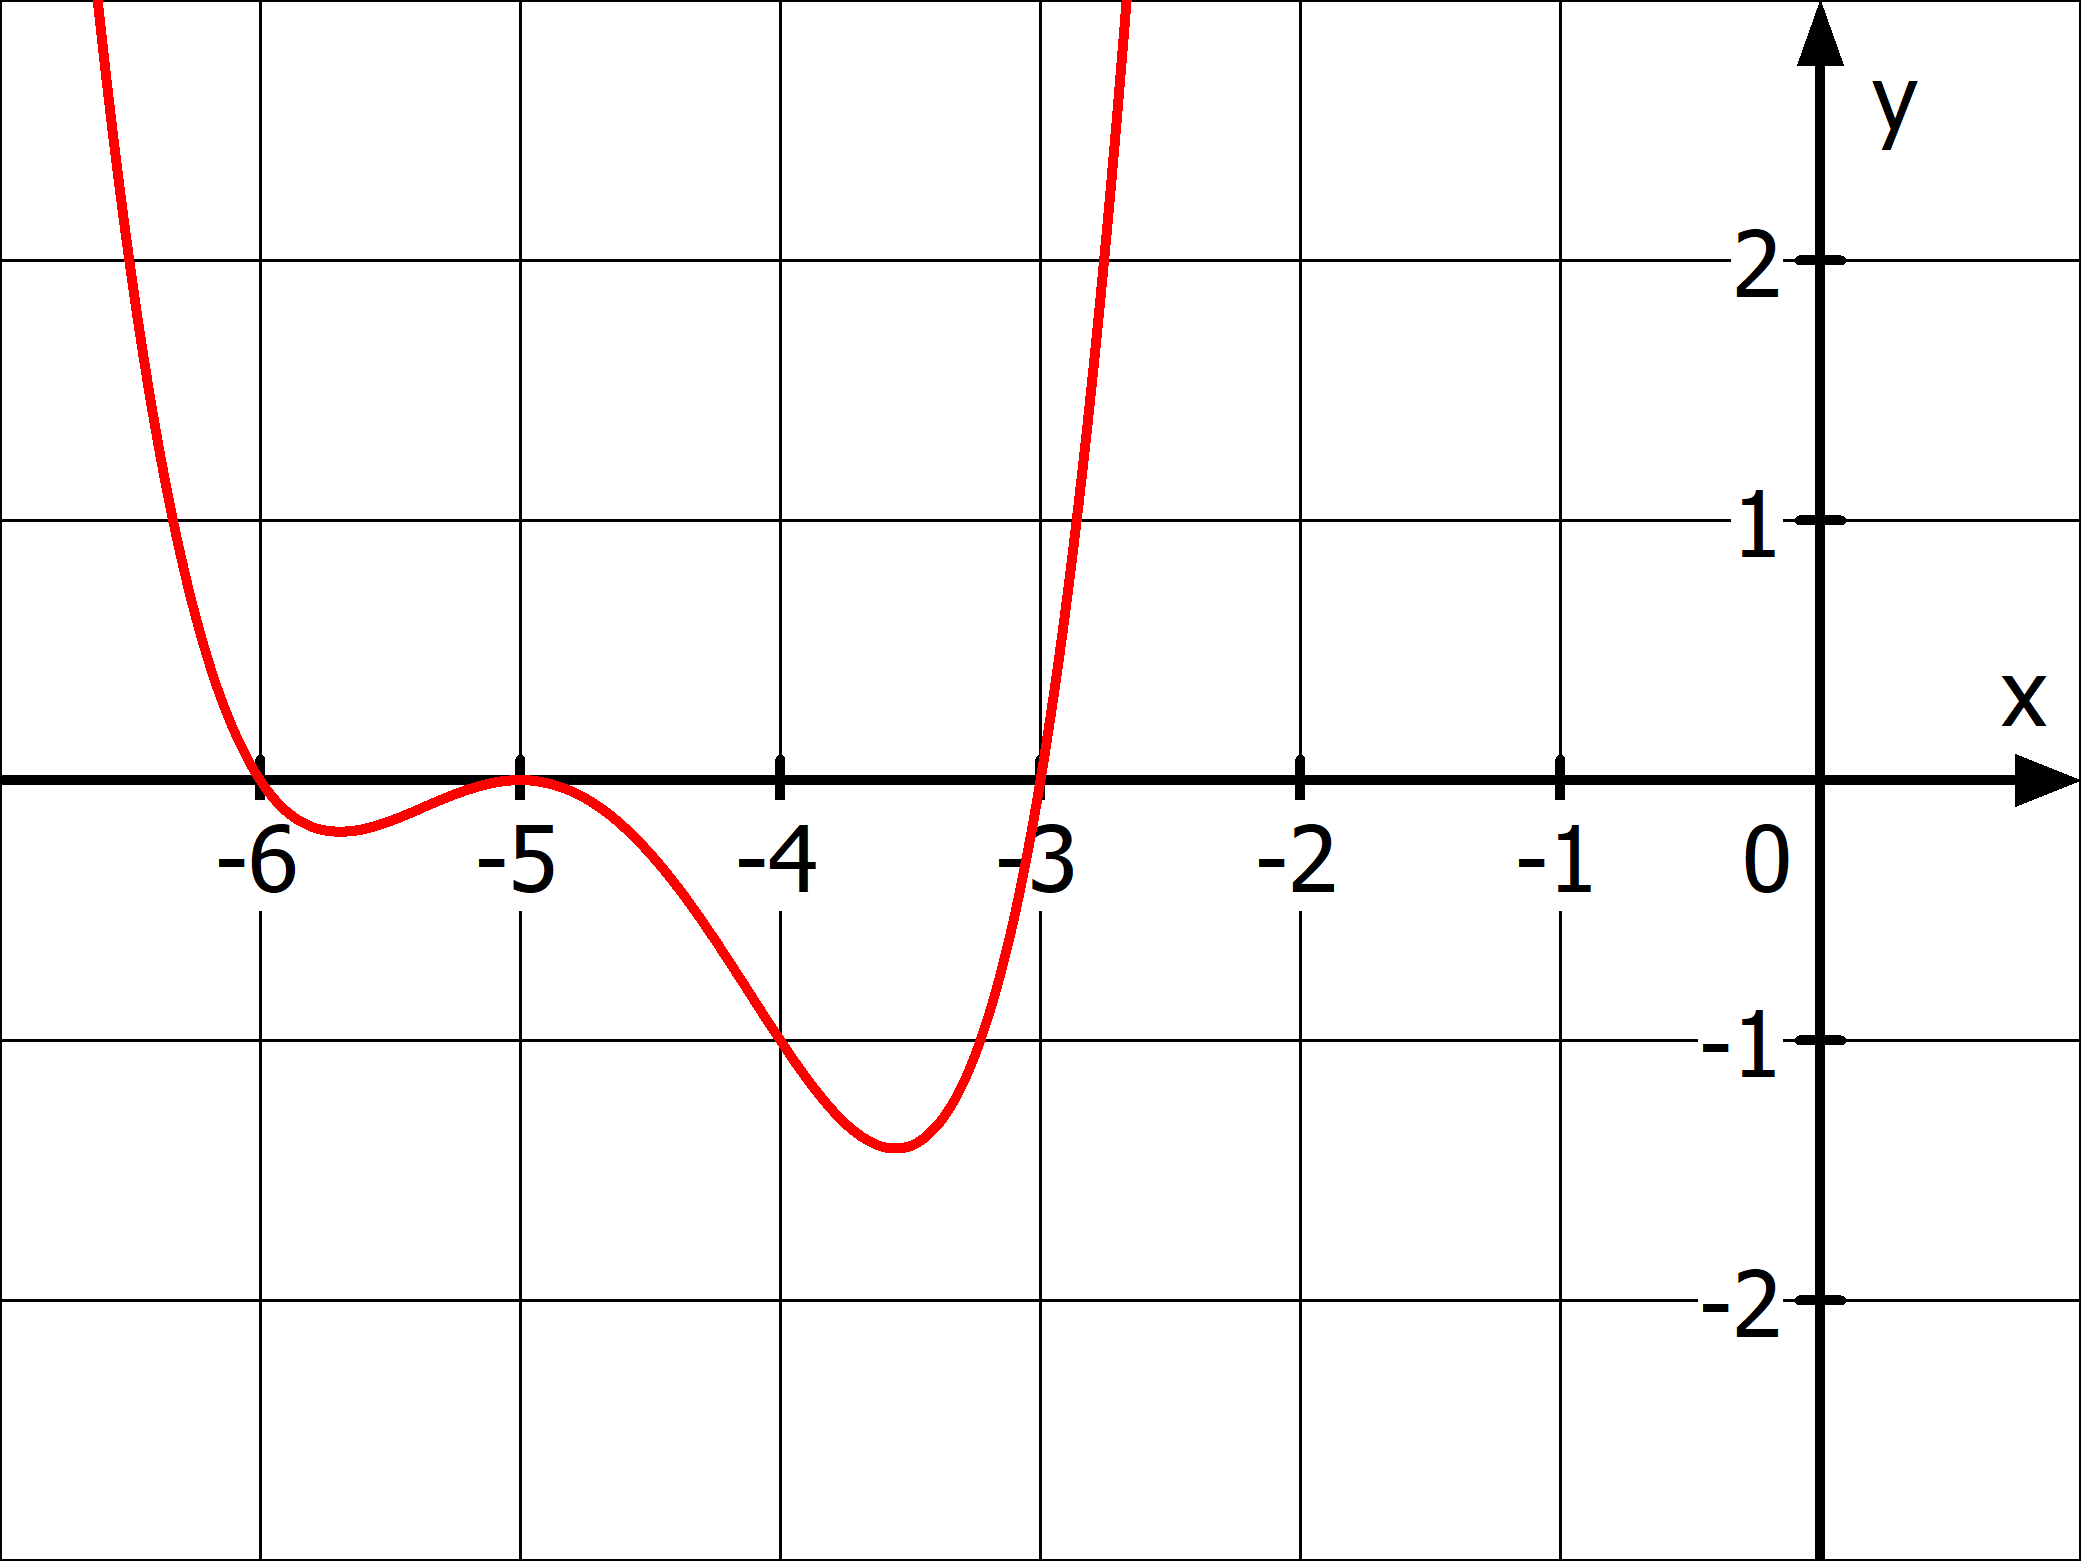
\includegraphics[width=\textwidth]{\ganzFkt/pics/produktA2_4.png}%
				\end{minipage}%

                \bigskip

				\item \begin{minipage}[t]{0.8\textwidth}\vspace{-0.5\baselineskip}
					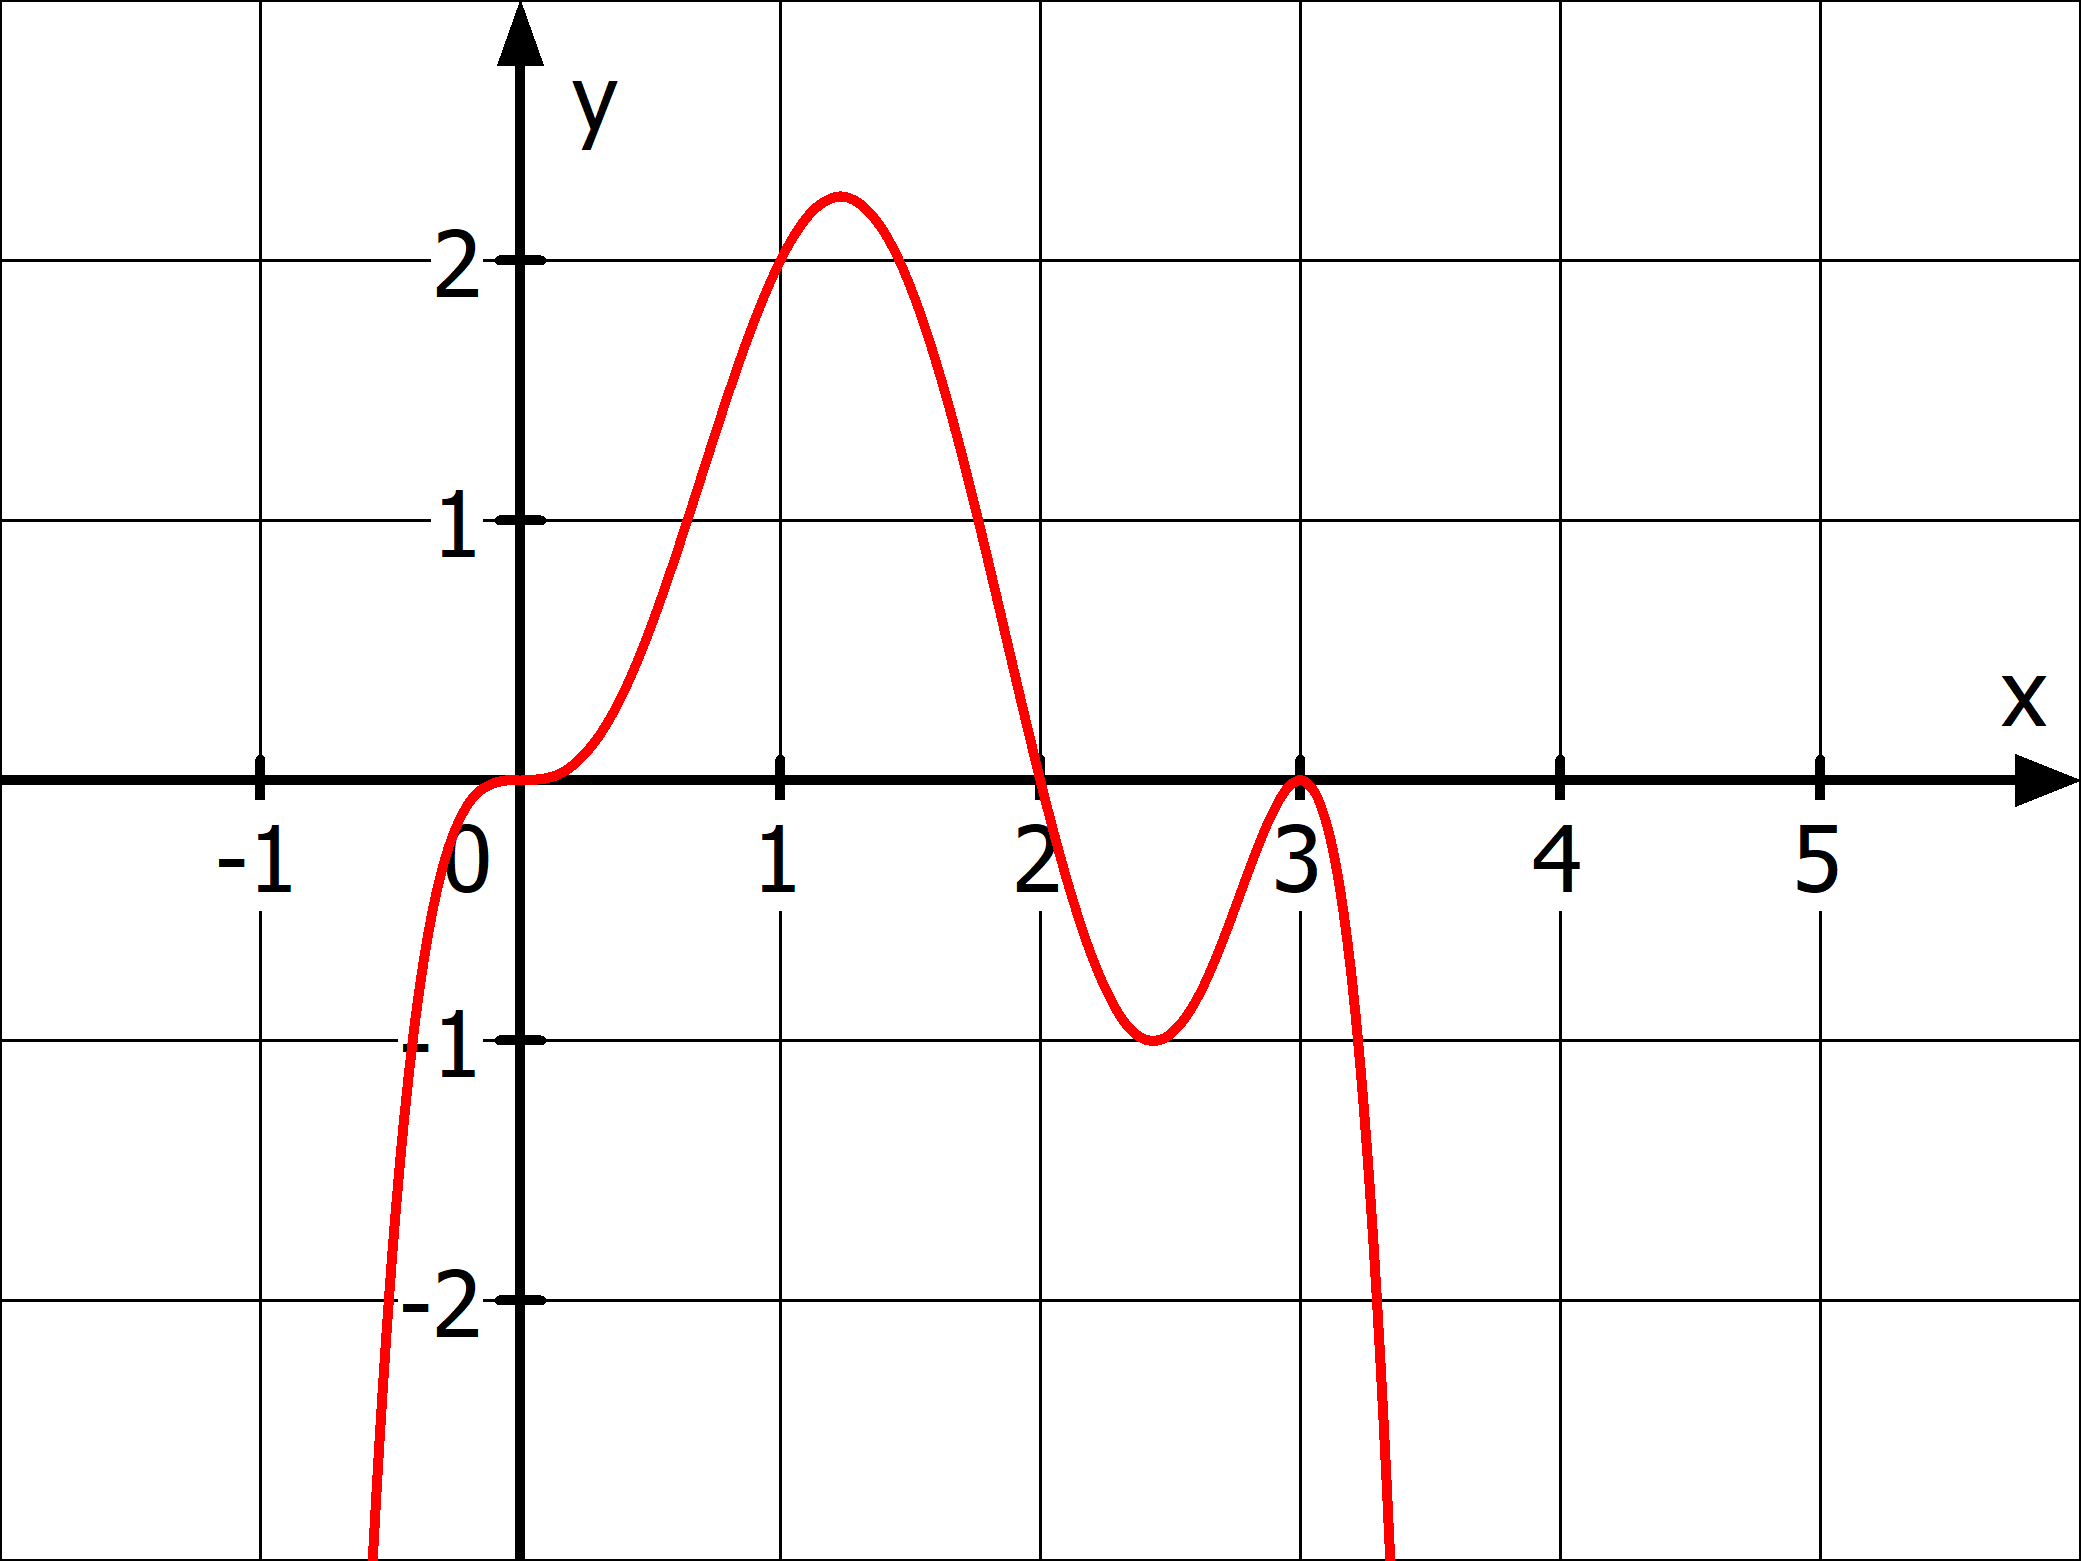
\includegraphics[width=\textwidth]{\ganzFkt/pics/produktA2_5.png}%
				\end{minipage}%

                \bigskip

				\item \begin{minipage}[t]{0.8\textwidth}\vspace{-0.5\baselineskip}
					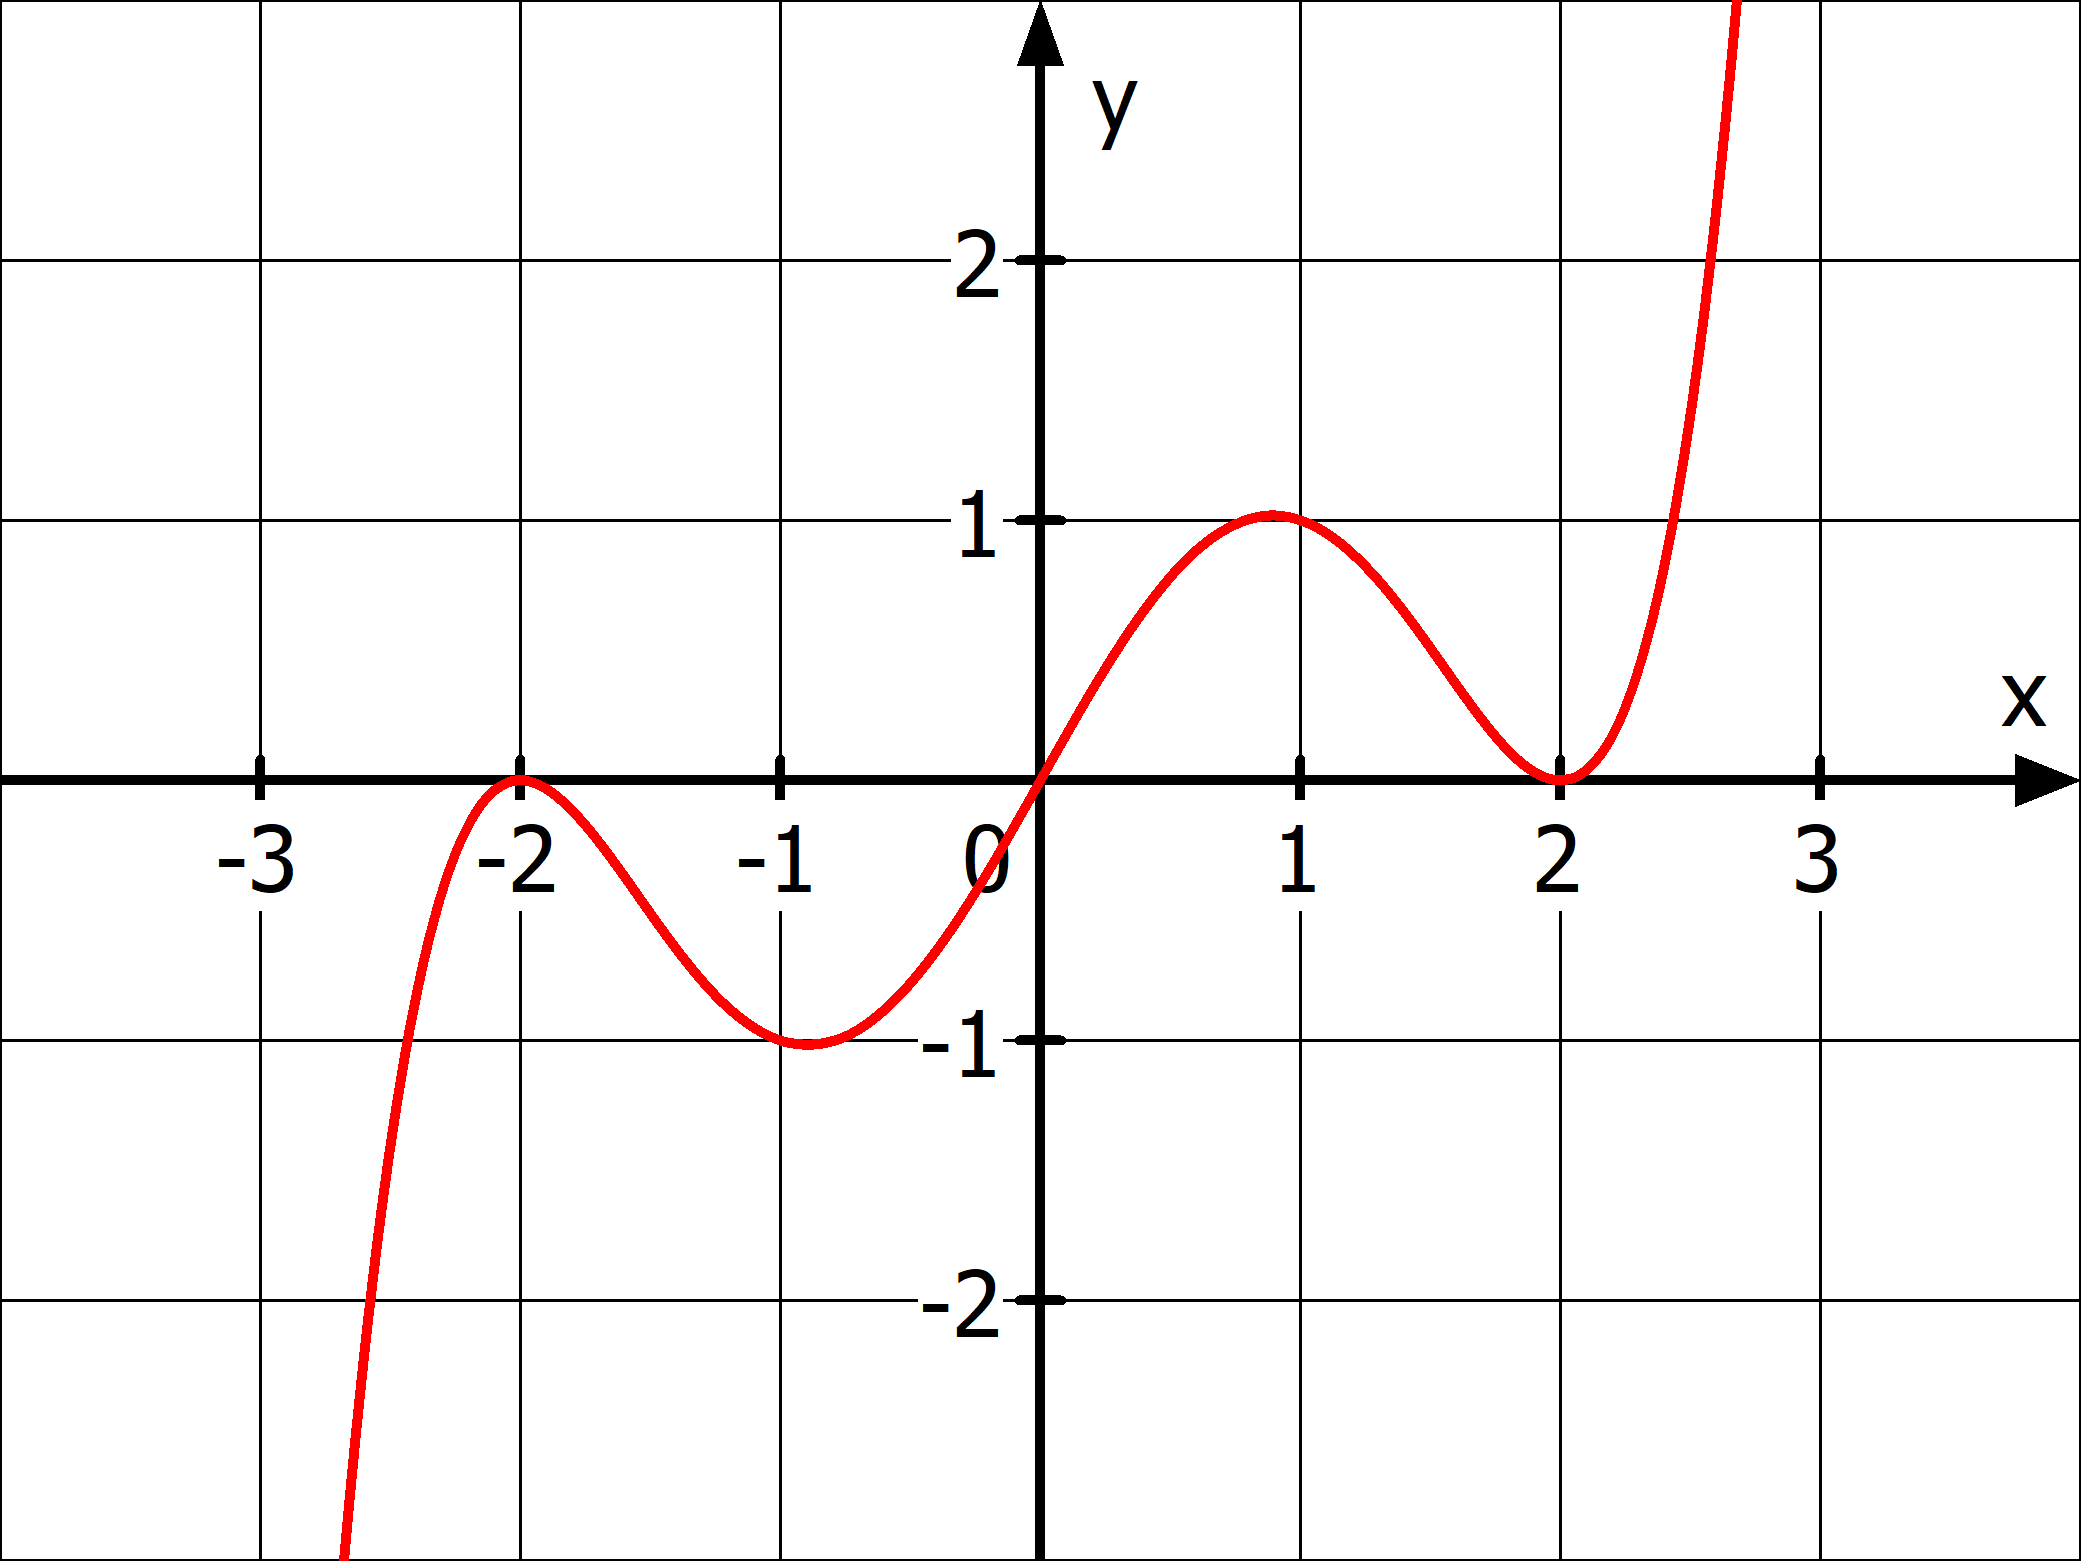
\includegraphics[width=\textwidth]{\ganzFkt/pics/produktA2_6.png}%
				\end{minipage}%
			\end{enumerate}%
		\end{minipage}%
	\end{minipage}%
\end{Exercise}\newpage
%%%%%%%%%%%%%%%%%%%%%%%%%%%%%%%%%%%%%%%%%%%%%%%%%%%%%%%%%%%%%%%%%%%%%%%
%%%%%%%%%%%%%%%%%%%%%%%%%%%%%%%%%%%%%%%%%
\begin{Answer}[ref=ganzProduktA1]

	\begin{minipage}{\textwidth}
		\begin{minipage}{0.5\textwidth}
			\begin{enumerate}[label=\alph*)]
				\item \(f(x)=0,1\left(x+3\right)^2\left(x+1\right)\left(x-1\right)^3\)

                \begin{minipage}[t]{0.8\textwidth}
					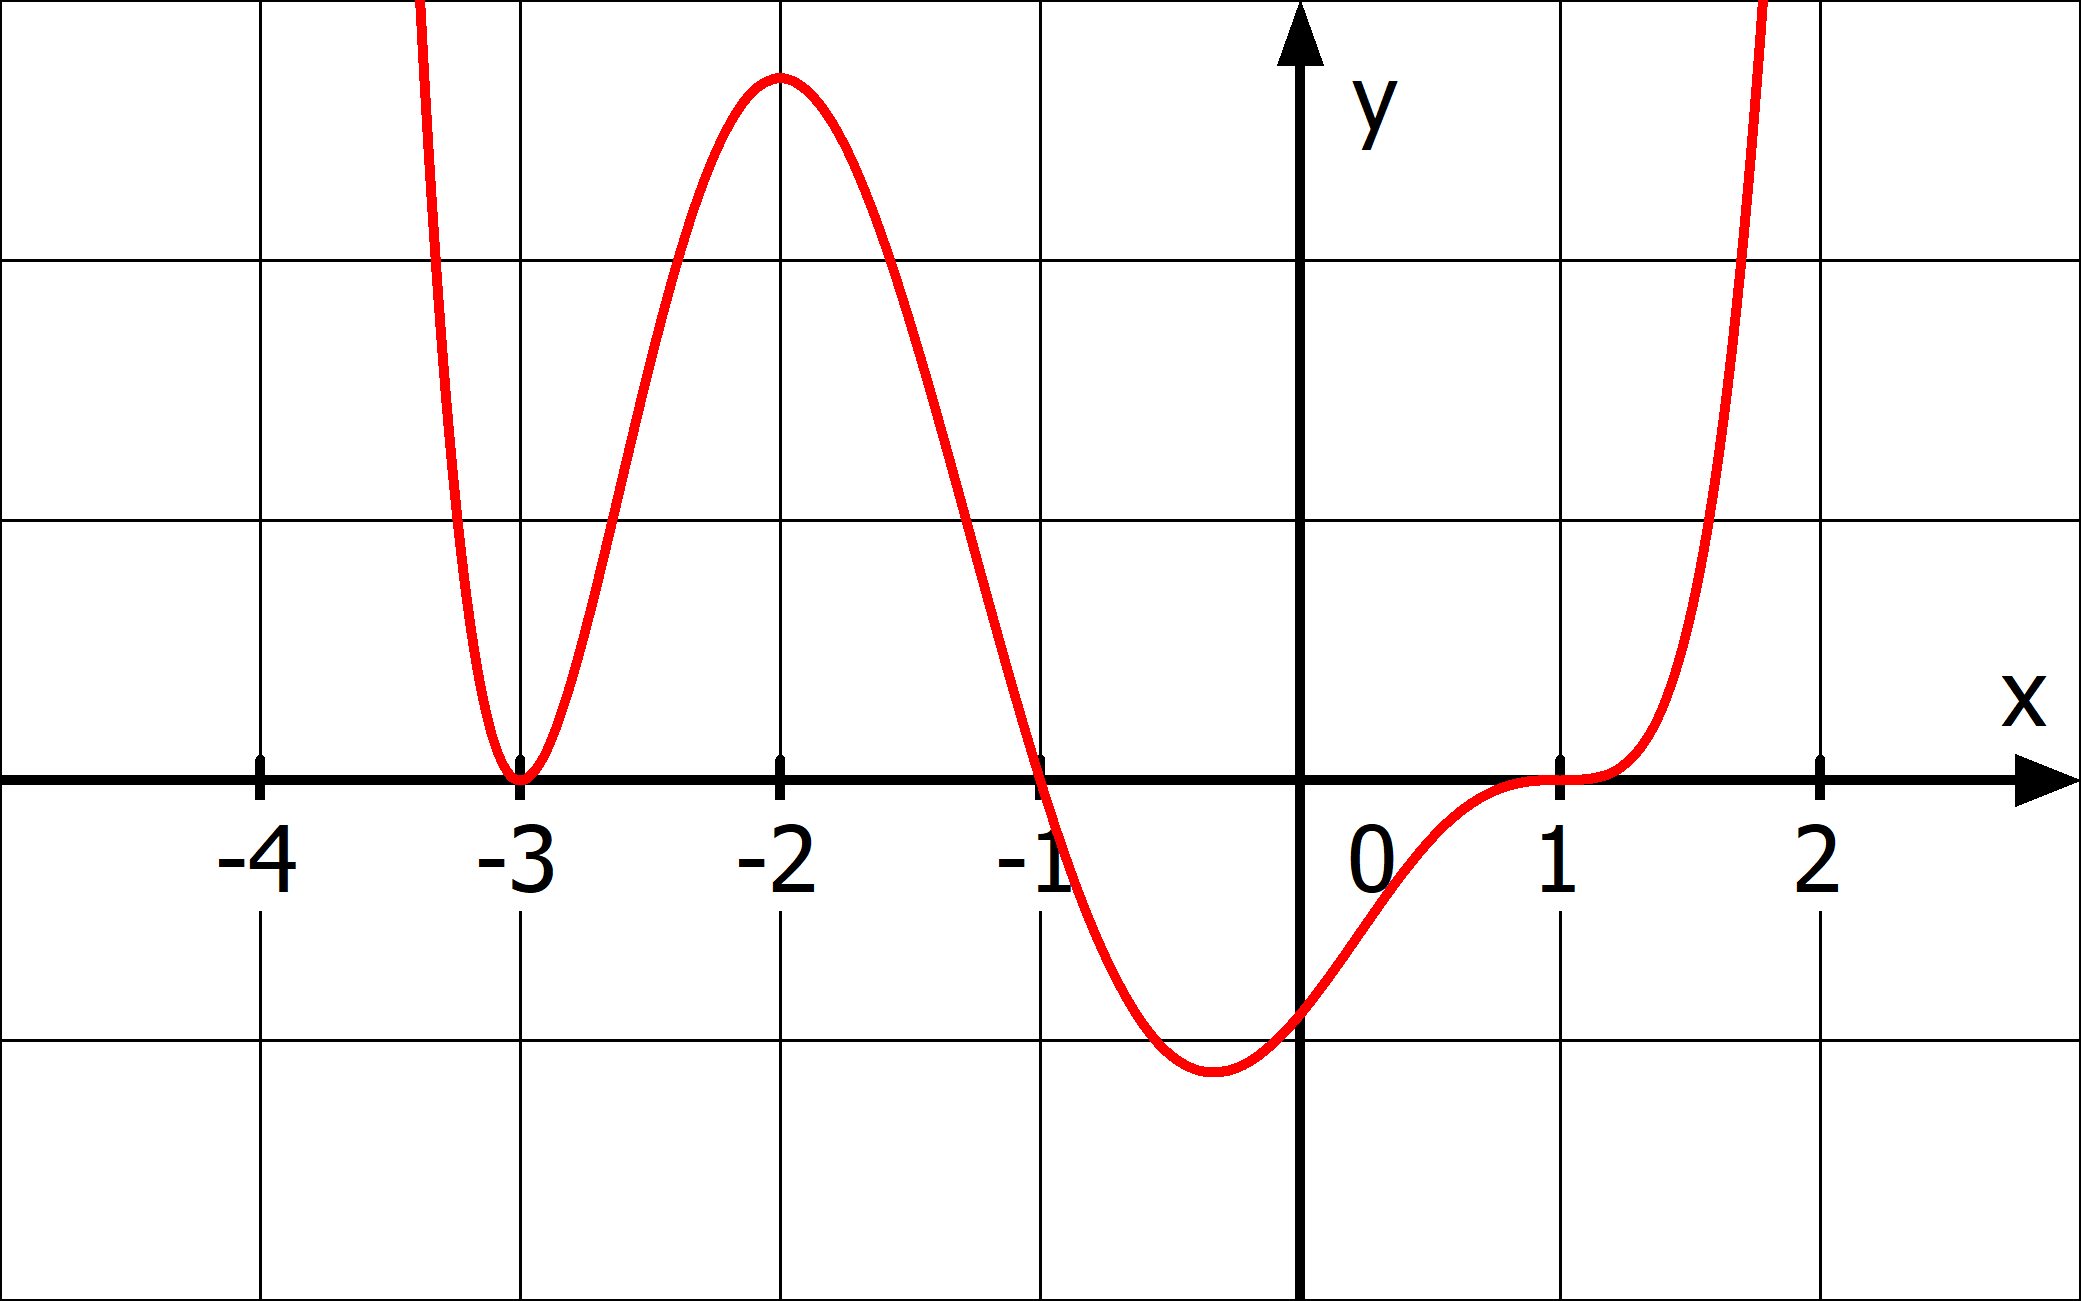
\includegraphics[width=\textwidth]{\ganzFkt/pics/produktA1_1.png}
				\end{minipage}%
				\item \(g(x)=-\frac{1}{5}\left(x+4\right) \left(x+3\right) \left(x+1\right) x^2 \)

                \begin{minipage}[t]{0.8\textwidth}
					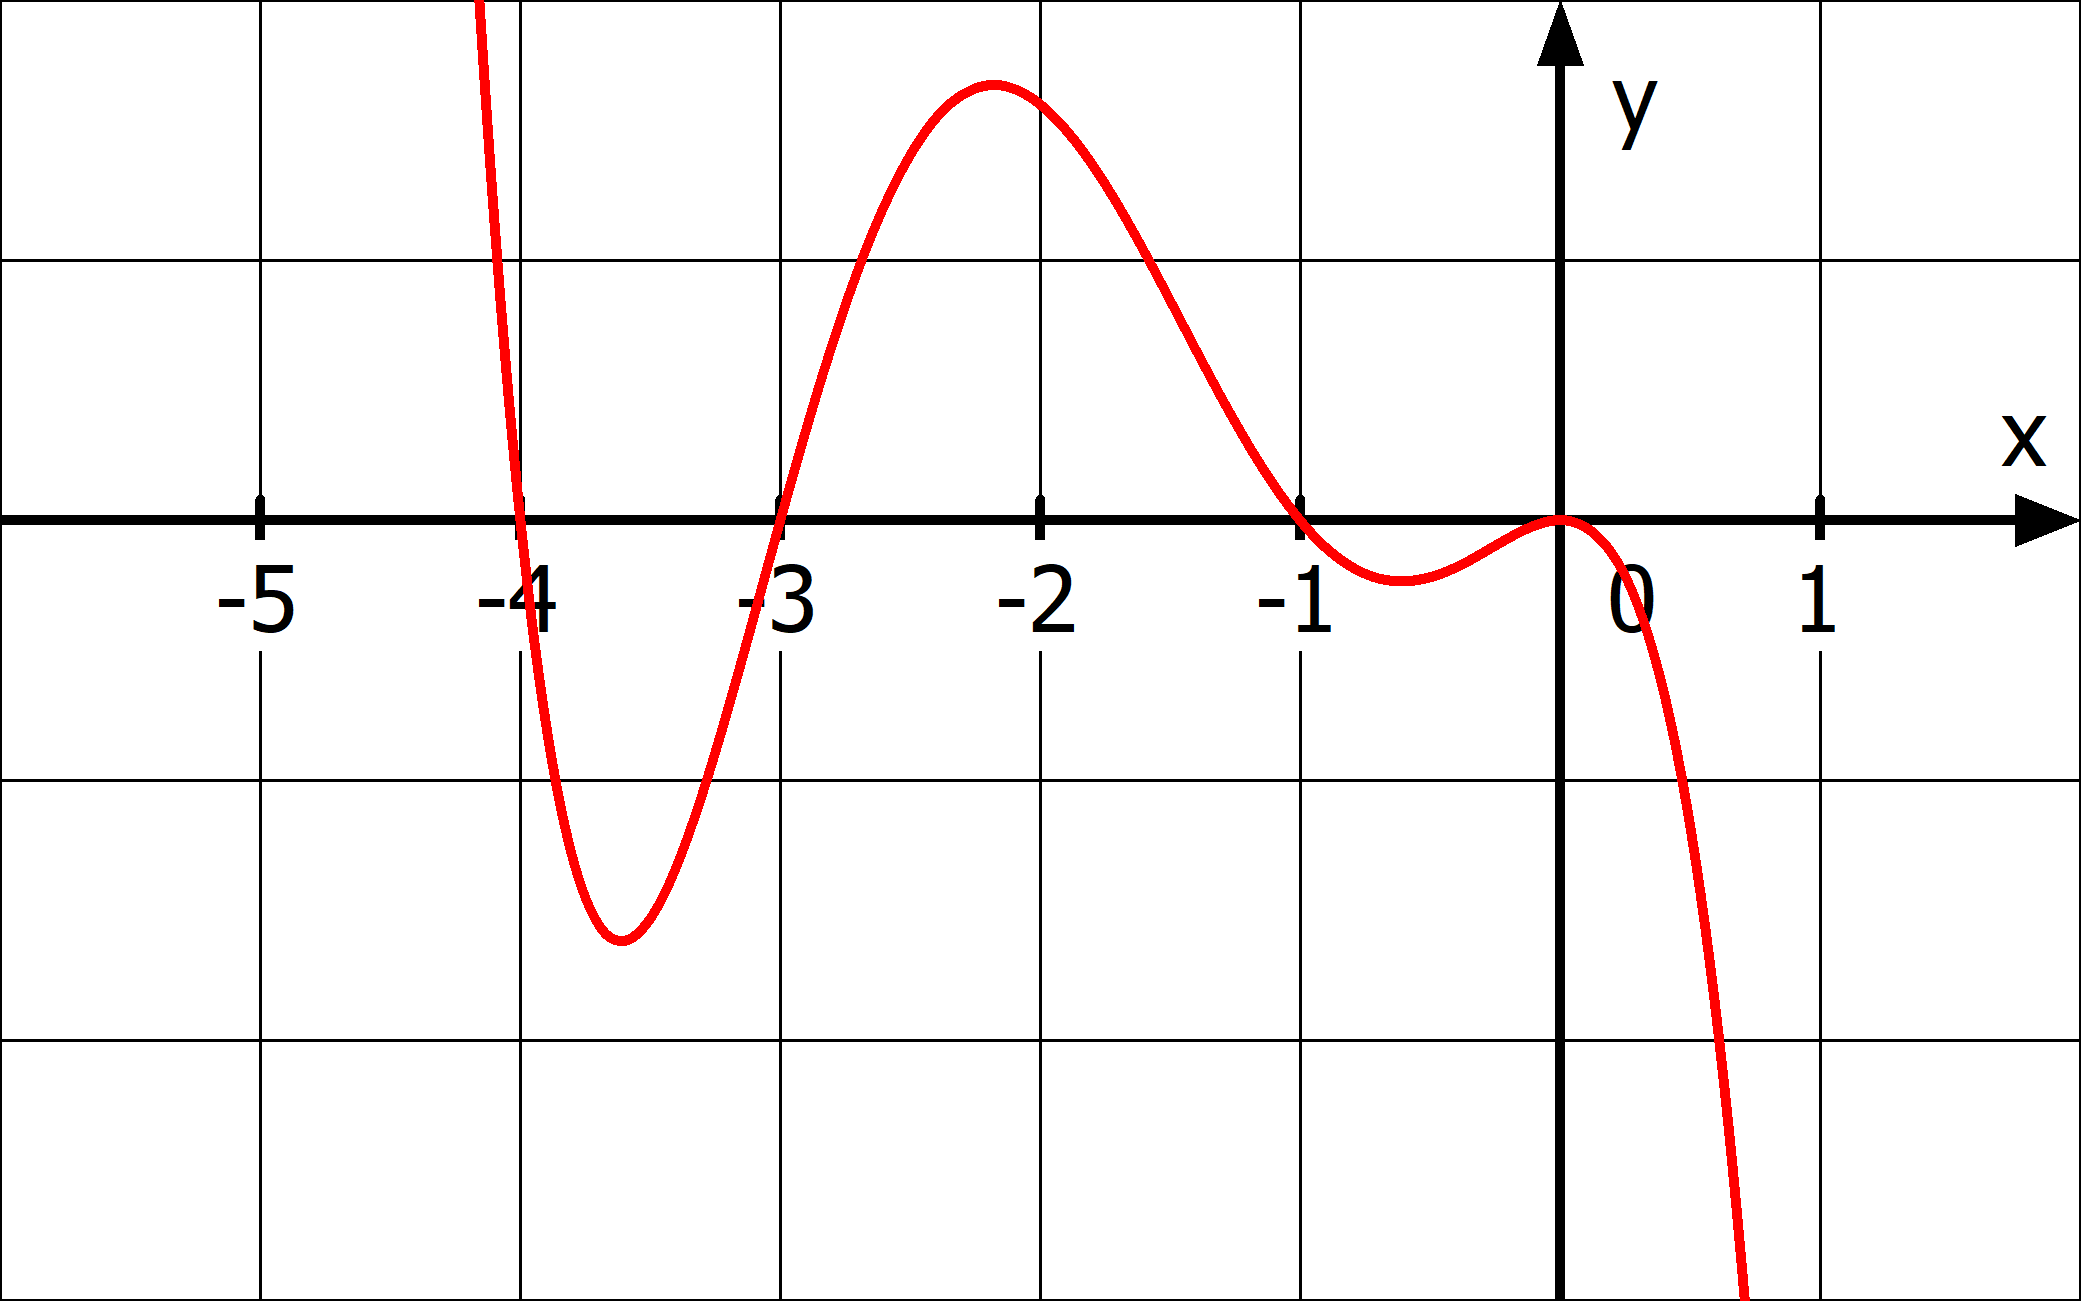
\includegraphics[width=\textwidth]{\ganzFkt/pics/produktA1_2.png}
				\end{minipage}%
				\item \(h(x)=-\left(x+1\right)^3 \left(x-1\right)^2 \left(x-2\right)\)

                \begin{minipage}[t]{0.8\textwidth}
					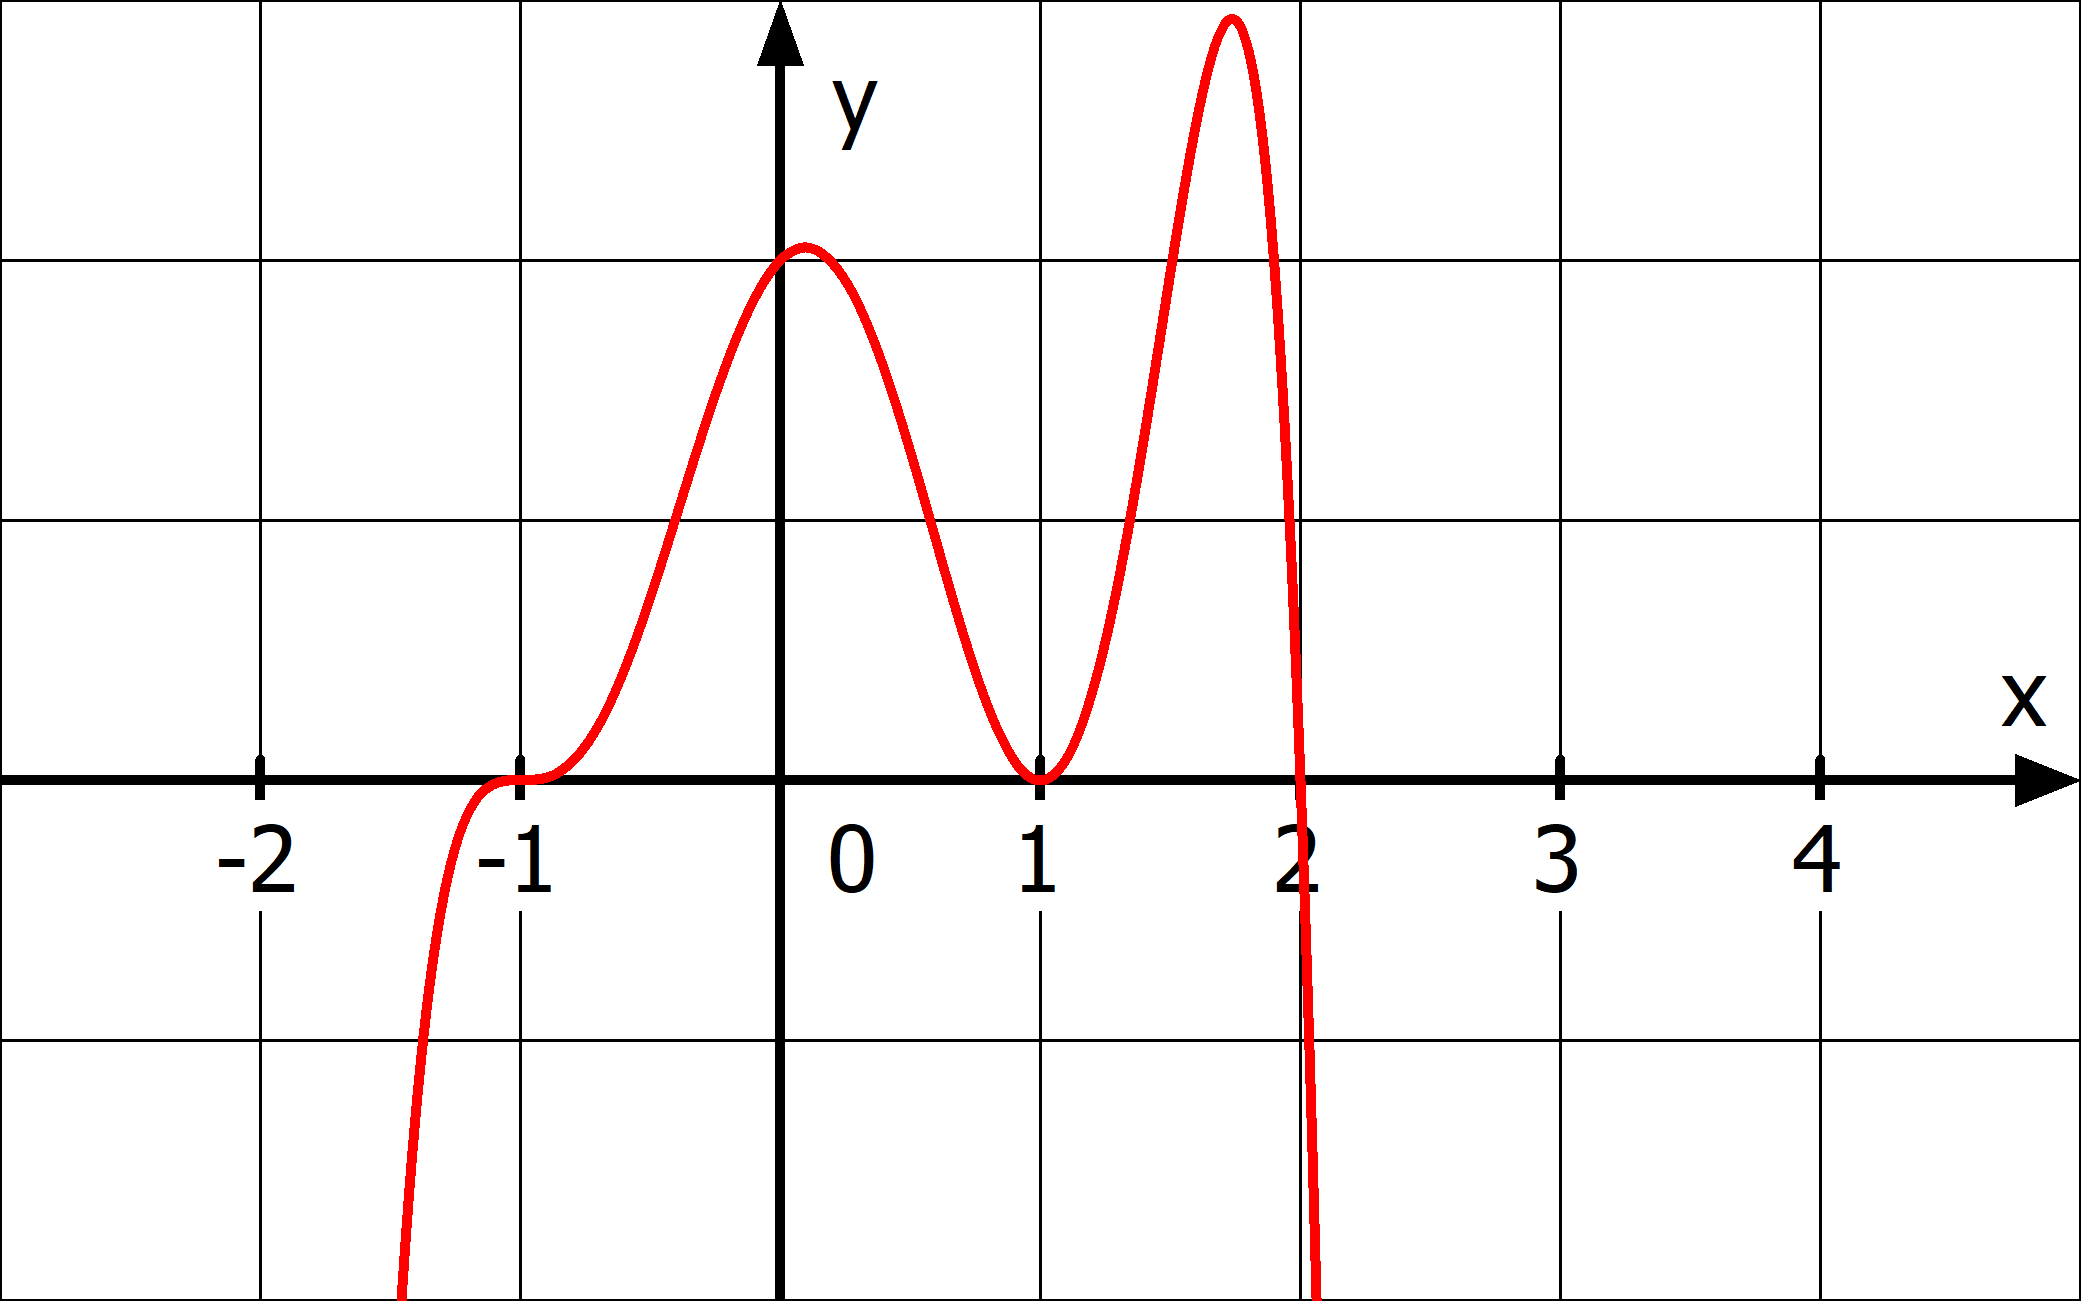
\includegraphics[width=\textwidth]{\ganzFkt/pics/produktA1_3.png}
				\end{minipage}%
				\item \(i(x)=\frac{1}{3}x^2\left(x+1\right) \left( x-2\right) \left( x-3\right) ^2\)

                \begin{minipage}[t]{0.8\textwidth}
					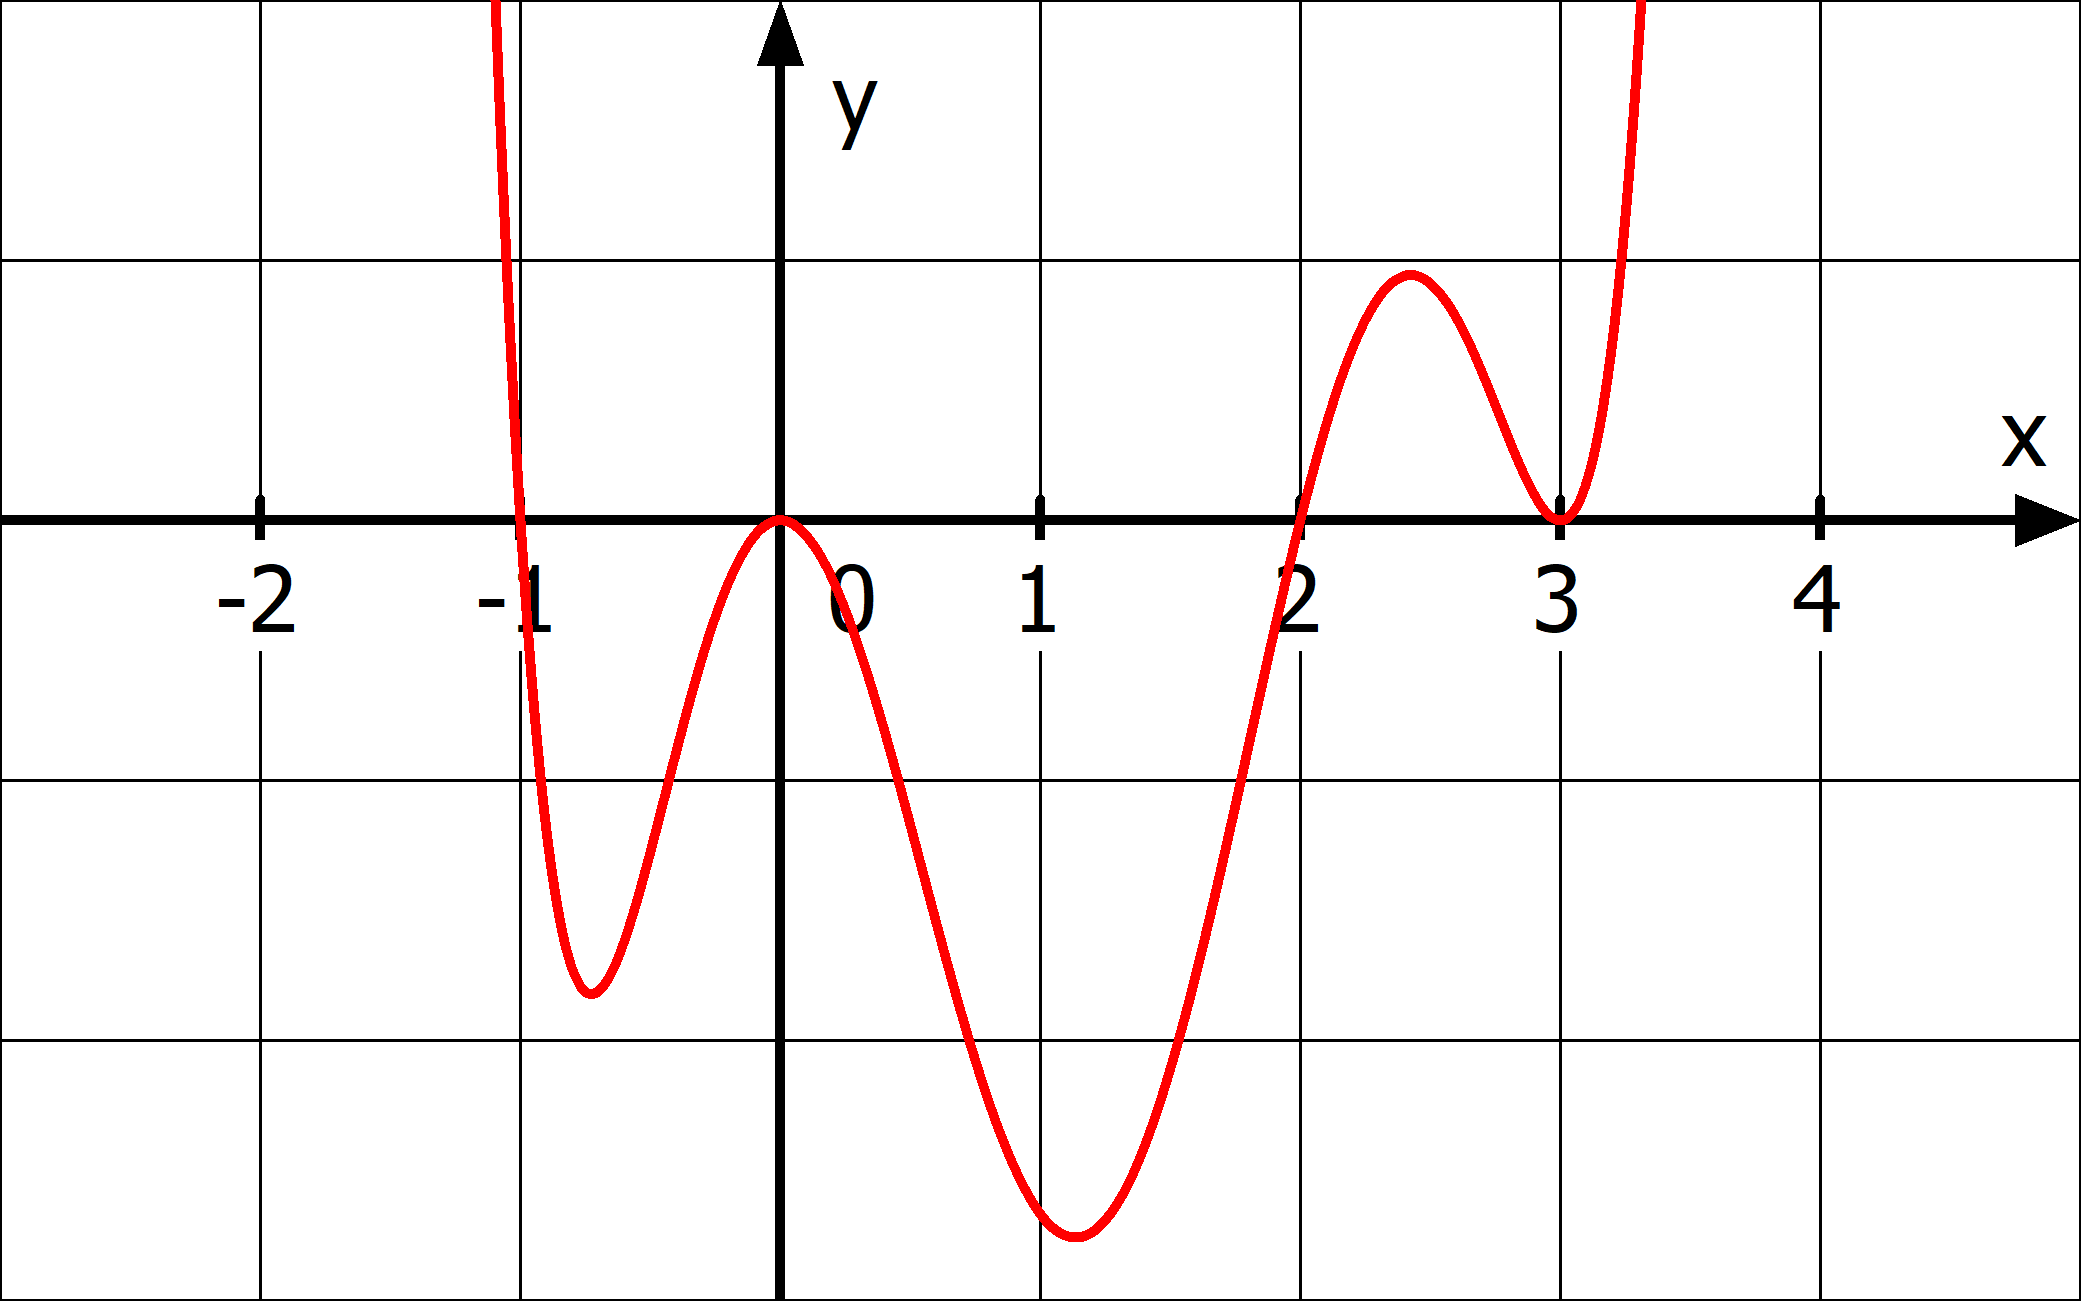
\includegraphics[width=\textwidth]{\ganzFkt/pics/produktA1_4.png}
				\end{minipage}%
			\end{enumerate}
		\end{minipage}%
		\begin{minipage}{0.5\textwidth}
			\begin{enumerate}[label=\alph*)]
				\setcounter{enumi}{4}
				\item \(j(x)=\frac{1}{5}\left( x+2\right) x\left( x-2\right) ^2\)

                \begin{minipage}[t]{0.8\textwidth}
					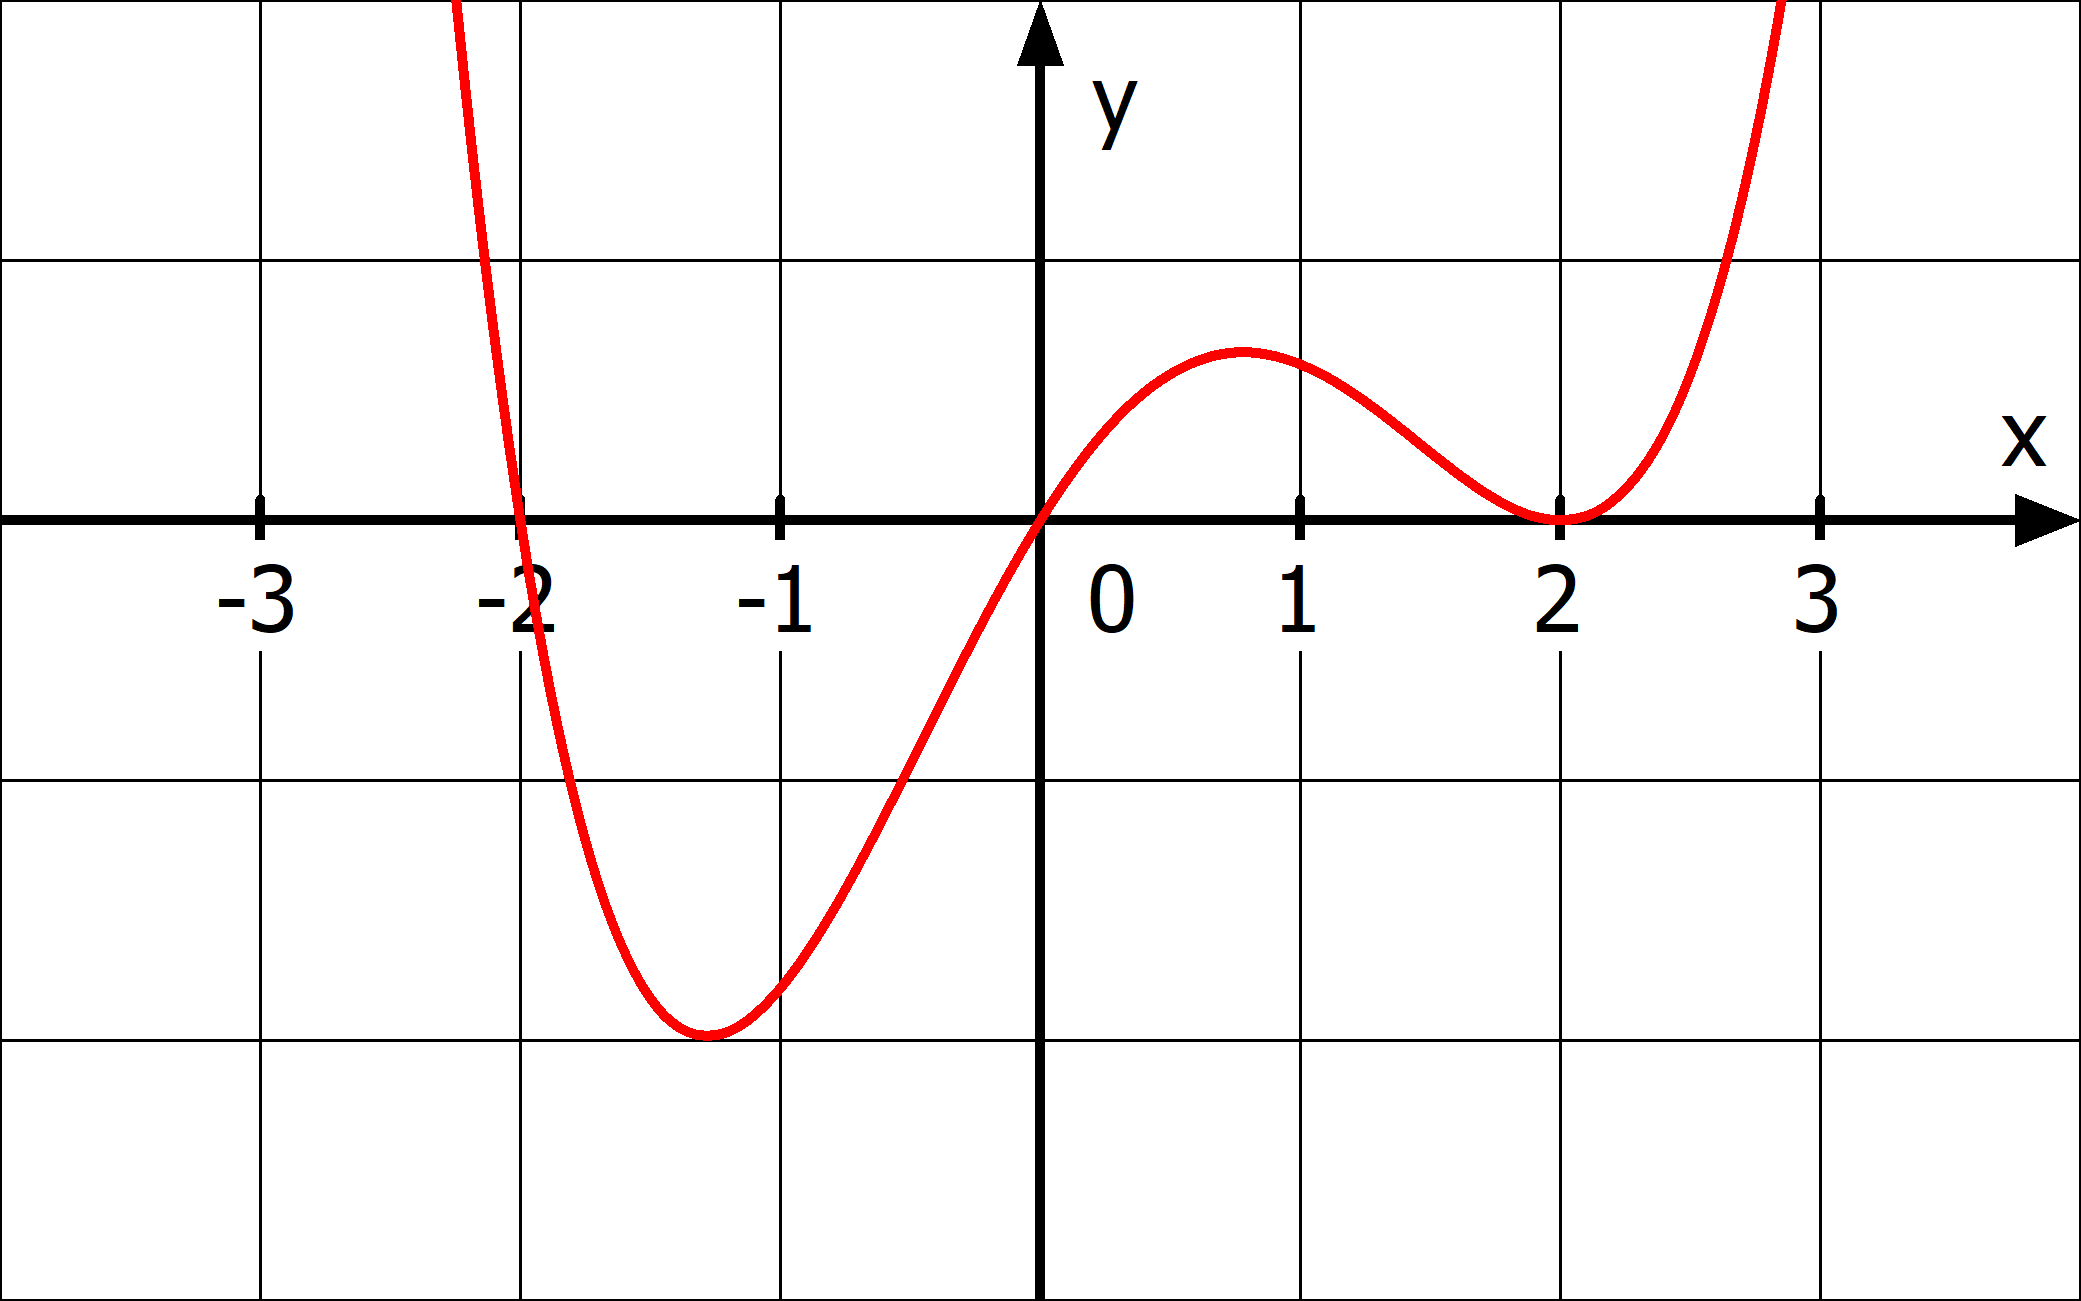
\includegraphics[width=\textwidth]{\ganzFkt/pics/produktA1_5.png}
				\end{minipage}%
				\item \(k(x)=-x^3\left( x-2\right) ^2\)

                \begin{minipage}[t]{0.8\textwidth}
					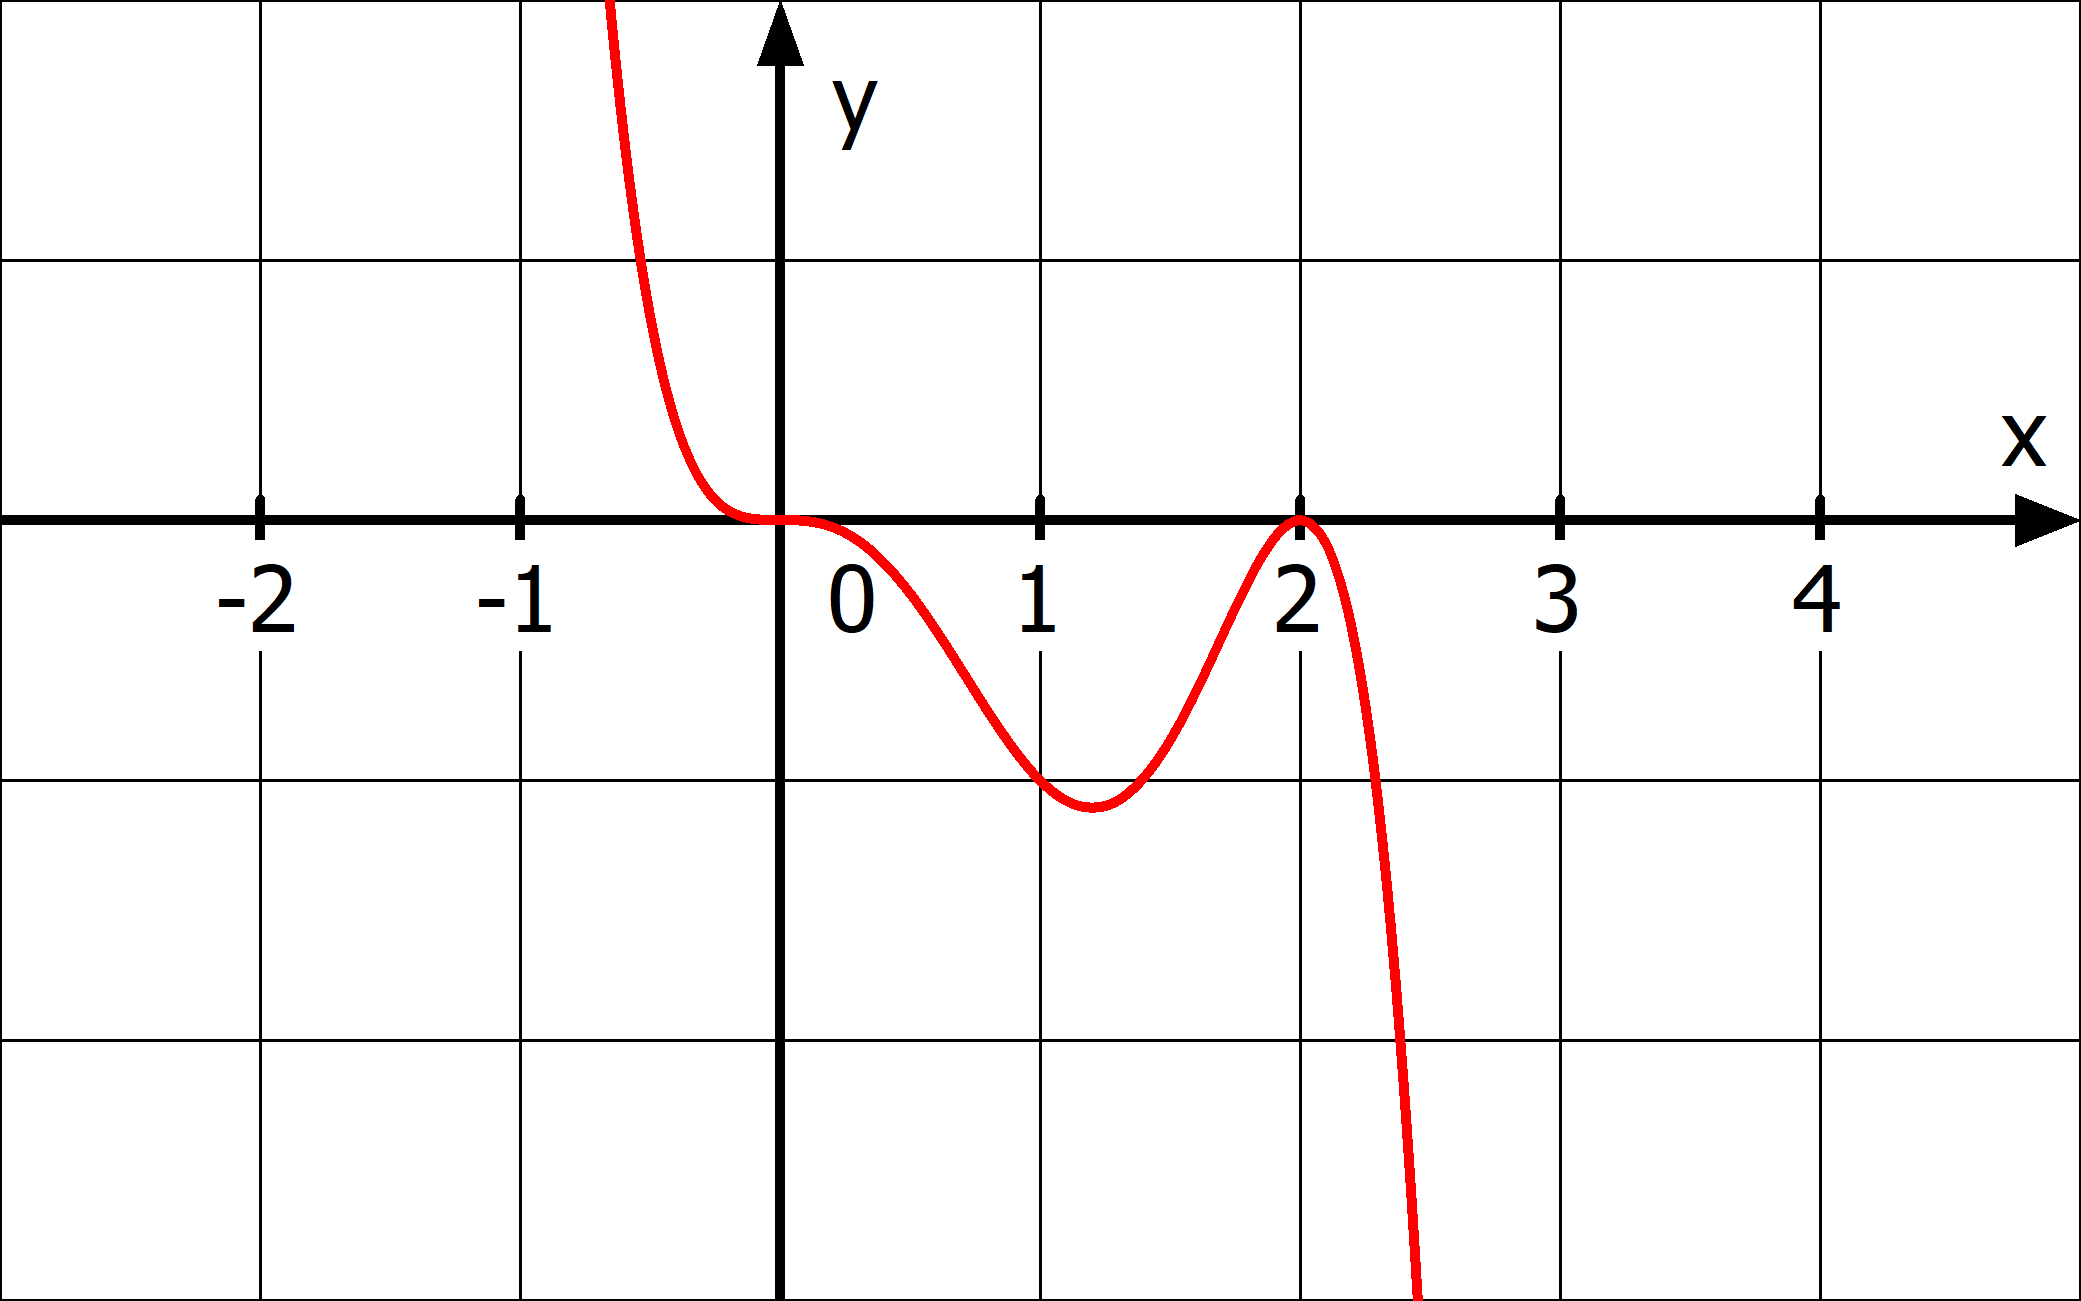
\includegraphics[width=\textwidth]{\ganzFkt/pics/produktA1_6.png}
				\end{minipage}%
				\item \(l(x)=\frac{1}{10}\left( x+4\right) ^2 x^2\)

                \begin{minipage}[t]{0.8\textwidth}
					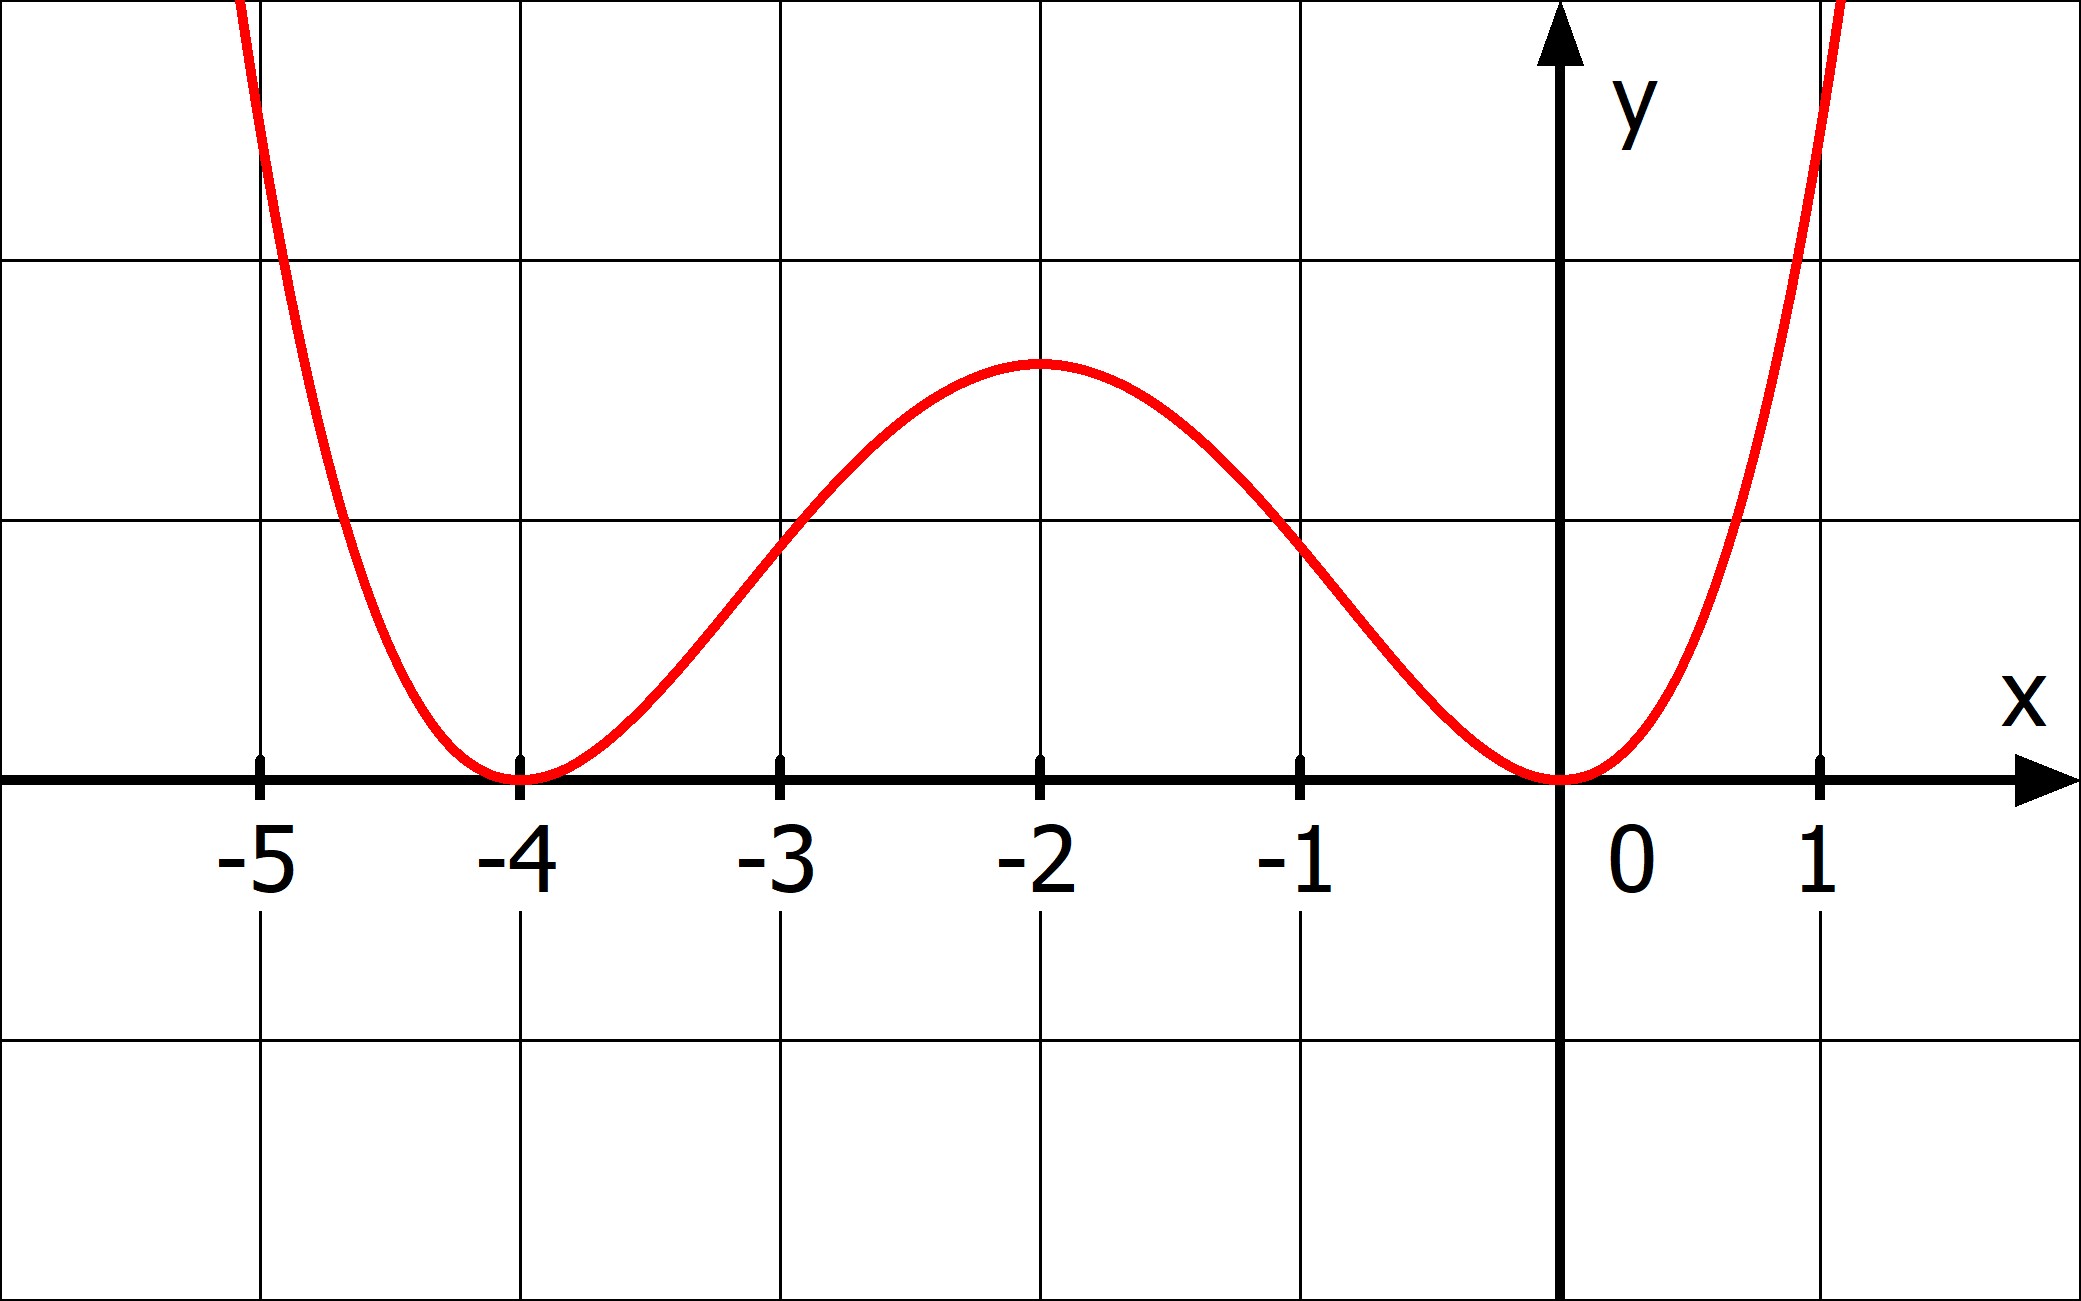
\includegraphics[width=\textwidth]{\ganzFkt/pics/produktA1_7.png}
				\end{minipage}%
				\item \(m(x)=-\frac{3}{35}\left( x+5\right) \left( x+4\right) ^2\left( x+2\right) x\)

                \begin{minipage}[t]{0.8\textwidth}
					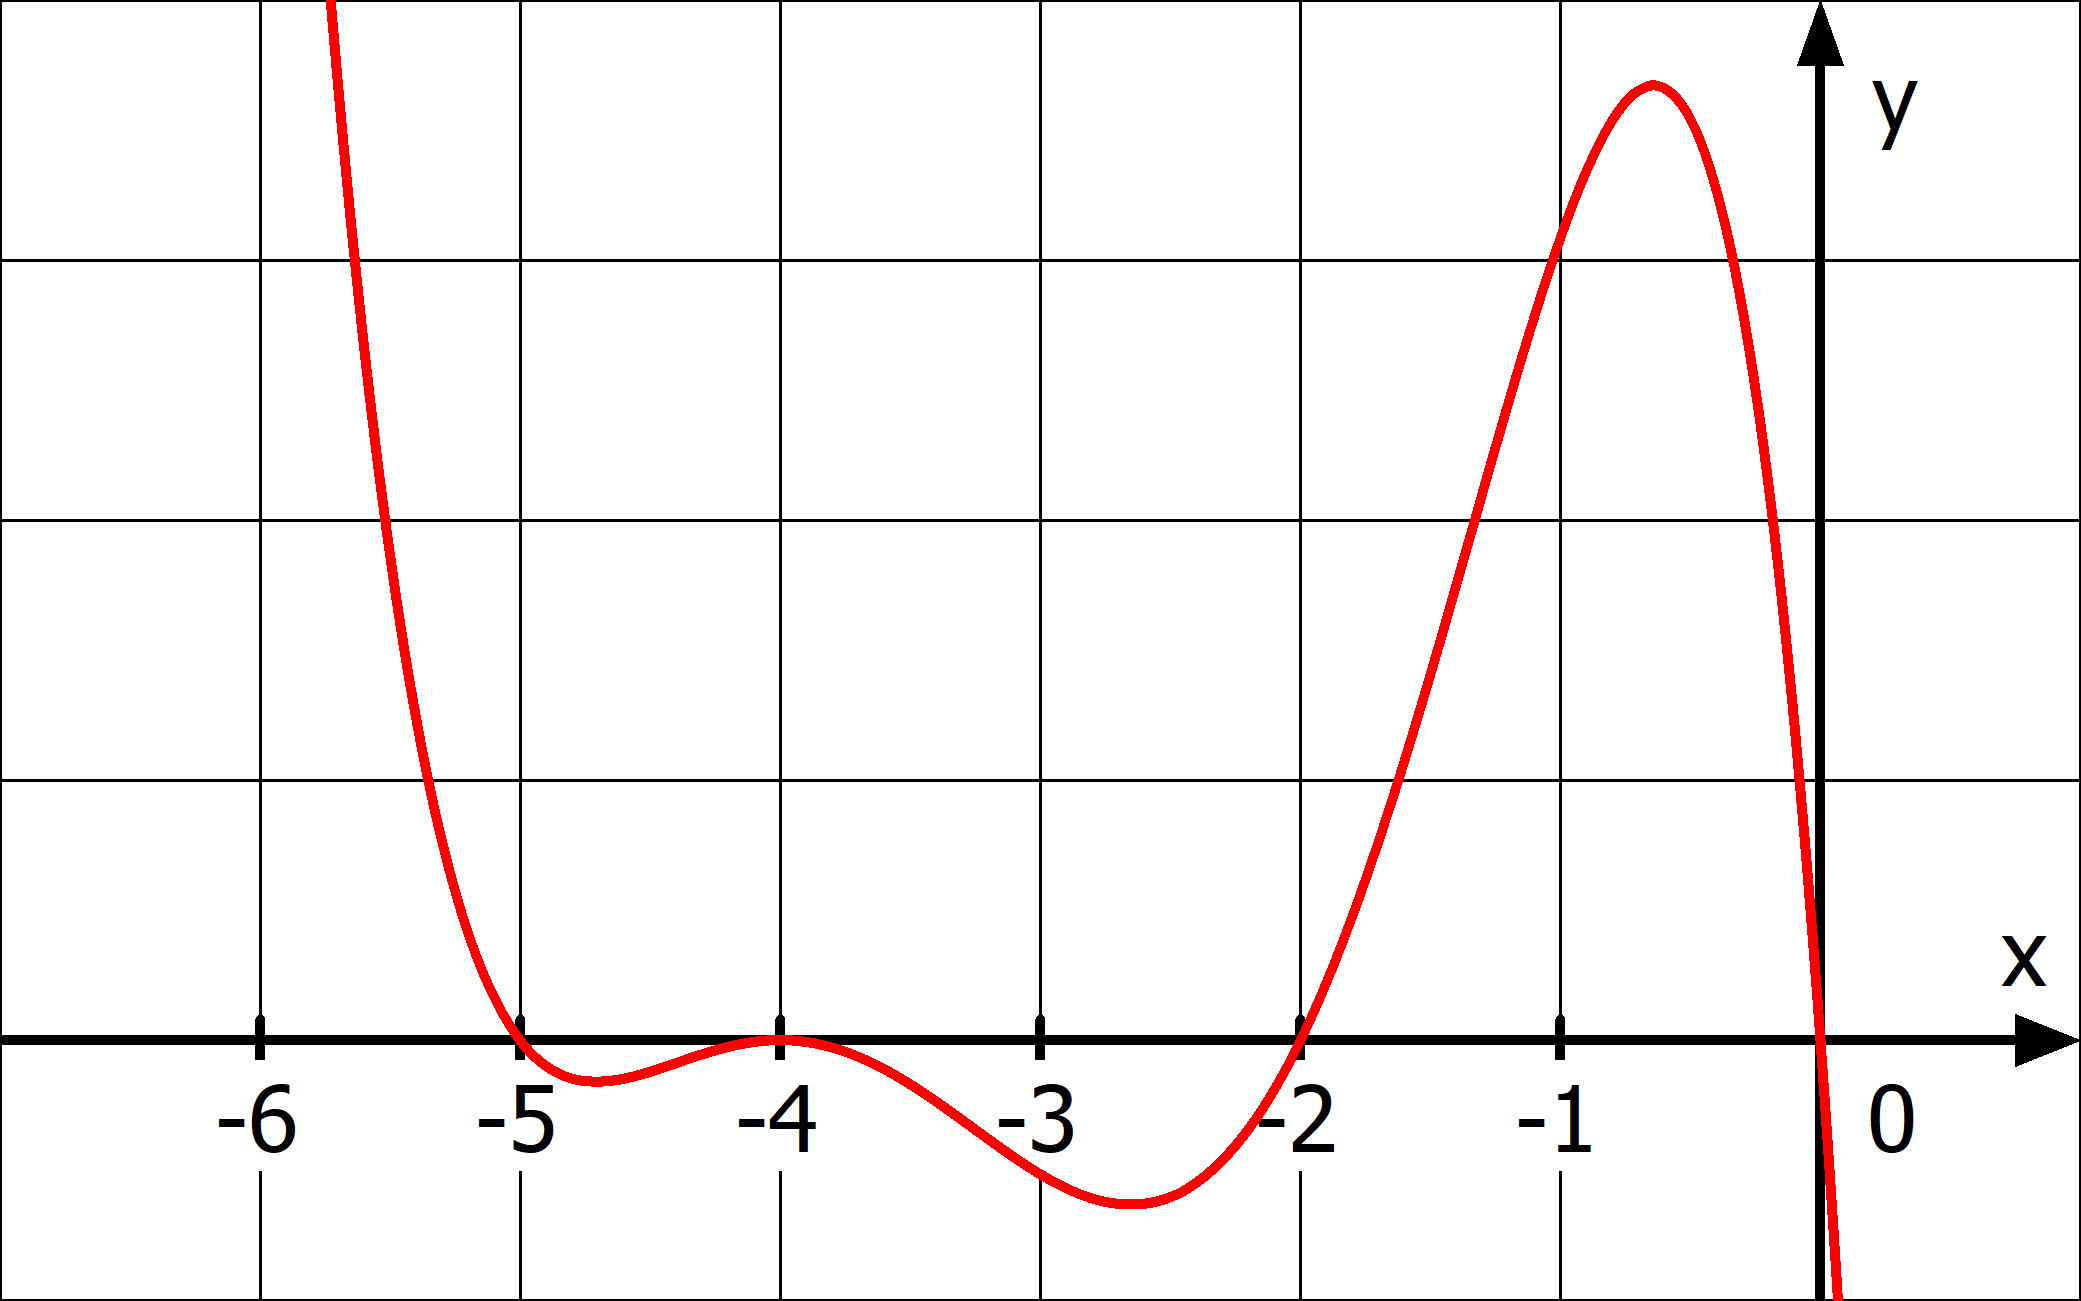
\includegraphics[width=\textwidth]{\ganzFkt/pics/produktA1_8.png}
				\end{minipage}%
			\end{enumerate}
		\end{minipage}%
	\end{minipage}%
\end{Answer}\newpage
\begin{Answer}[ref=ganzProduktA2]

	\begin{minipage}{\textwidth}
		\begin{minipage}[t]{0.5\textwidth}
			\begin{enumerate}[label=\alph*)]
				\item \(f_a(x)=-\frac{1}{6}\left(x+4\right) \left(x+2\right) \left(x-1\right)^2 \)
				\item \(f_b(x)=\left(x+2\right)x^3\left(x-1\right) \)
				\item \(f_c(x)=-\frac{3}{2}x^2\left(x-2\right)^2 \left(x-3\right) \)
			\end{enumerate}
		\end{minipage}%
		\begin{minipage}[t]{0.5\textwidth}
			\begin{enumerate}[label=\alph*)]
				\setcounter{enumi}{3}
				\item \(f_d(x)=\frac{1}{2}\left(x+6\right) \left(x+5\right)^2 \left(x+3\right) \)
				\item \(f_e(x)=-\frac{1}{2}x^3\left(x-2\right) \left(x-3\right)^2 \)
				\item \(f_f(x)=\frac{1}{9}\left(x+2\right)^2 x\left(x-2\right)^2 \)
			\end{enumerate}
		\end{minipage}%
	\end{minipage}%
\end{Answer}